\documentclass[a4paper,12pt]{article}
\usepackage[utf8]{inputenc}
\usepackage[LGR,T1]{fontenc}
\usepackage{alphabeta}
\usepackage{amsmath}
\usepackage{float}
\usepackage{multirow}
\usepackage{amsfonts}
\usepackage{amssymb}
\usepackage{graphicx}
\usepackage{listings}
\usepackage{booktabs}  % For better looking tables
\usepackage{hyperref}
\usepackage{xcolor}
\usepackage{breakurl}
\usepackage[numbers]{natbib}
\usepackage{subcaption}  % Προσθέστε αυτή τη γραμμή στο preample του εγγράφου

\lstset{
  basicstyle=\ttfamily\footnotesize,
  keywordstyle=\color{blue},
  commentstyle=\color{gray},
  stringstyle=\color{red},
  showstringspaces=false,
  breaklines=true,
  frame=single,
  language=R,
  extendedchars=true,
  literate={β}{{\beta}}1
}

\title{Αναγνώριση Προτύπων \\ 2η Εργαστηριακή Άσκηση \\ Χειμερινό Εξάμηνο 2024-2025 \\ Ε.ΔE.ΜΜ}
\author{Σπανάκης Παναγιώτης-Αλέξιος (ΑΜ: 03400274)}
\date{08/11/2024}

\begin{document}

\maketitle

\section*{Βήμα 1: Εξοικείωση με φασματογραφήματα στην κλίμακα mel}

\subsection*{α, β, γ) Ανάλυση των φασματογραφημάτων Mel}
Εξετάζοντας τα δύο παραδείγματα (Rock - Αρχείο 104085 και Electronic - Αρχείο 1334), παρατηρούμε τα εξής διακριτά χαρακτηριστικά:

\textbf{Είδος Rock (Αρχείο 104085):}
\begin{itemize}
    \item Υψηλότερο ενεργειακό περιεχόμενο σε όλο το εύρος συχνοτήτων (0-10000 Hz)
    \item Έντονη παρουσία στις μεσαίες συχνότητες (2000-6000 Hz)
    \item Σαφή κατακόρυφα μοτίβα που υποδεικνύουν τακτικά ρυθμικά στοιχεία
    \item Σταθερή ενέργεια στις χαμηλές συχνότητες που δείχνει έντονη παρουσία μπάσου/ντραμς
    \item Πιο ομοιόμορφη κατανομή ενέργειας που υποδηλώνει χρήση παραδοσιακών οργάνων
\end{itemize}

\textbf{Είδος Electronic (Αρχείο 1334):}
\begin{itemize}
    \item Συγκέντρωση ενέργειας στις χαμηλές συχνότητες (0-4000 Hz)
    \item Λιγότερο ομοιόμορφη φασματική κατανομή
    \item Πιο σποραδικά μοτίβα στις υψηλές συχνότητες
    \item Μεταβλητά χρονικά μοτίβα τυπικά των συνθετικών ήχων
    \item Λιγότερο καθορισμένες κατακόρυφες γραμμές, υποδεικνύοντας διαφορετικές ρυθμικές δομές
\end{itemize}

\subsection*{δ) Η Κλίμακα Mel}
Η κλίμακα Mel είναι μια αντιληπτική κλίμακα συχνοτήτων που αναπτύχθηκε για να ταιριάζει με τον τρόπο που οι άνθρωποι αντιλαμβάνονται τις διαφορές τόνου.

\textbf{1. Ορισμός και Δημιουργία:}
\begin{itemize}
    \item Δημιουργήθηκε μέσω πειραμάτων όπου οι ακροατές αναγνώριζαν ζεύγη ήχων που αντιλαμβάνονταν ως ισαπέχοντα σε τόνο
    \item Τύπος: $mel = 2595 \cdot \log_{10}(1 + \frac{f}{700})$, όπου f η συχνότητα σε Hz
    \item Περίπου γραμμική κάτω από 1000 Hz και λογαριθμική πάνω από αυτή
\end{itemize}

\textbf{2. Χρήση στην Επεξεργασία Μουσικής:}
\begin{itemize}
    \item Καλύτερη αναπαράσταση της ανθρώπινης ακουστικής αντίληψης
    \item Παρέχει μεγαλύτερη ανάλυση στις χαμηλές συχνότητες όπου η ανθρώπινη ακοή είναι πιο ευαίσθητη
    \item Μειώνει την υπολογιστική πολυπλοκότητα διατηρώντας τις αντιληπτικά σημαντικές πληροφορίες
    \item Βελτιώνει την απόδοση στην ταξινόμηση και ανάλυση μουσικής
\end{itemize}

\section*{Βήμα 2: Συγχρονισμός φασματογραφημάτων στο ρυθμό της μουσικής}

\subsection*{α) Ανάλυση Διαστάσεων}

\textbf{Διαστάσεις Φασματογραφημάτων:}
\begin{itemize}
    \item Τα αρχικά φασματογραφήματα έχουν περίπου 1291-1293 χρονικά βήματα
    \item Κάθε χρονικό βήμα περιέχει 140 χαρακτηριστικά (128 για mel + 12 για chroma)
\end{itemize}

\textbf{Αποδοτικότητα LSTM:}
\begin{itemize}
    \item Η εκπαίδευση LSTM με τόσα πολλά χρονικά βήματα δεν είναι αποδοτική για τους εξής λόγους:
          \begin{enumerate}
              \item \textbf{Υπολογιστική Πολυπλοκότητα:}
                    \begin{itemize}
                        \item Τα LSTM πρέπει να επεξεργαστούν κάθε χρονικό βήμα διαδοχικά
                        \item Μεγάλες ακολουθίες αυξάνουν σημαντικά τον χρόνο εκπαίδευσης
                        \item Απαιτούν περισσότερη μνήμη για την αποθήκευση των ενδιάμεσων καταστάσεων
                    \end{itemize}

              \item \textbf{Πρόβλημα Εξαφανιζόμενης Κλίσης:}
                    \begin{itemize}
                        \item Μεγάλες ακολουθίες επιδεινώνουν το πρόβλημα των εξαφανιζόμενων κλίσεων
                        \item Δυσκολεύουν την εκμάθηση μακροπρόθεσμων εξαρτήσεων
                    \end{itemize}

              \item \textbf{Περιττή Πληροφορία:}
                    \begin{itemize}
                        \item Πολλά διαδοχικά χρονικά βήματα μπορεί να περιέχουν παρόμοια πληροφορία
                        \item Δεν είναι απαραίτητη τόσο λεπτομερής χρονική ανάλυση για την ταξινόμηση είδους
                    \end{itemize}
          \end{enumerate}
\end{itemize}

\subsection*{β) Ανάλυση Beat-Synchronized Φασματογραφημάτων}

\textbf{Σύγκριση με τα Αρχικά Φασματογραφήματα:}
\begin{itemize}
    \item \textbf{Πλεονεκτήματα:}
          \begin{enumerate}
              \item \textbf{Μειωμένη Διάσταση:}
                    \begin{itemize}
                        \item Σημαντικά λιγότερα χρονικά βήματα
                        \item Πιο αποδοτική επεξεργασία και εκπαίδευση
                    \end{itemize}

              \item \textbf{Μουσική Σημασία:}
                    \begin{itemize}
                        \item Ευθυγράμμιση με τη ρυθμική δομή της μουσικής
                        \item Καλύτερη αναπαράσταση των μουσικών γεγονότων
                    \end{itemize}

              \item \textbf{Ποιότητα Χαρακτηριστικών:}
                    \begin{itemize}
                        \item Διατήρηση των σημαντικών φασματικών χαρακτηριστικών
                        \item Μείωση του θορύβου μέσω της διαμέσου
                    \end{itemize}
          \end{enumerate}

    \item \textbf{Διαφορές στην Οπτικοποίηση:}
          \begin{itemize}
              \item Πιο ευδιάκριτα ρυθμικά μοτίβα
              \item Καλύτερη αναπαράσταση της μουσικής δομής
              \item Ομαλότερη χρονική εξέλιξη των χαρακτηριστικών
          \end{itemize}
\end{itemize}

\textbf{Συμπέρασμα:}
Ο συγχρονισμός με το ρυθμό προσφέρει μια πιο συμπαγή και μουσικά σημαντική αναπαράσταση, κατάλληλη για εκπαίδευση νευρωνικών δικτύων, διατηρώντας παράλληλα τα ουσιώδη χαρακτηριστικά για την ταξινόμηση του μουσικού είδους.

\section*{Βήμα 3: Εξοικείωση με χρωμογραφήματα}

Αναλύοντας τα χρωμογραφήματα για τα ίδια δύο αρχεία παρατηρούμε διαφορετικά αρμονικά χαρακτηριστικά:

\textbf{Είδος Rock (Αρχείο 104085):}
\begin{itemize}
    \item Σαφής αρμονική δομή με καθορισμένα μοτίβα νοτών
    \item Έντονη παρουσία σε συγκεκριμένες τάξεις τόνου (κυρίως E)
    \item Τακτικά μοτίβα που υποδεικνύουν σταθερές ακολουθίες συγχορδιών
    \item Καλά καθορισμένες μεταβάσεις μεταξύ διαφορετικού αρμονικού περιεχομένου
\end{itemize}

\textbf{Είδος Electronic (Αρχείο 1334):}
\begin{itemize}
    \item Πιο διάχυτη κατανομή ενέργειας στις τάξεις τόνου
    \item Έντονη δραστηριότητα στην περιοχή της νότας A
    \item Λιγότερο καθορισμένες αρμονικές ακολουθίες
    \item Θολές μεταβάσεις μεταξύ νοτών
\end{itemize}

\textbf{Βασικές Παρατηρήσεις για τα Χρωμογραφήματα:}
\begin{enumerate}
    \item \textbf{Αναπαράσταση:}
          \begin{itemize}
              \item Δείχνει την κατανομή ενέργειας στις 12 τάξεις τόνου (C έως B)
              \item Συμπτύσσει τις πληροφορίες οκτάβας για εστίαση στο αρμονικό περιεχόμενο
              \item Η φωτεινότητα υποδεικνύει την ένταση κάθε τάξης τόνου
          \end{itemize}

    \item \textbf{Οφέλη Μουσικής Ανάλυσης:}
          \begin{itemize}
              \item Αποκαλύπτει την αρμονική δομή ανεξάρτητα από την οκτάβα
              \item Ανθεκτικό στις αλλαγές ηχοχρώματος διατηρώντας τις αρμονικές πληροφορίες
              \item Χρήσιμο για την ανάλυση ακολουθιών συγχορδιών
              \item Βοηθά στην αναγνώριση τονικότητας και τροπικού περιεχομένου
          \end{itemize}
\end{enumerate}

Οι εκδόσεις συγχρονισμένες με το ρυθμό (beat-synchronized) ευθυγραμμίζουν αυτά τα χαρακτηριστικά με το μουσικό παλμό, καθιστώντας τα χρονικά μοτίβα πιο εμφανή και ευκολότερα στην ανάλυση.

\section*{Βήμα 4: Φόρτωση και ανάλυση δεδομένων}

\subsection*{α) Ανάλυση Κώδικα PyTorch Dataset}

Ο κώδικας υλοποιεί τις εξής βασικές λειτουργίες:

\begin{enumerate}
    \item \textbf{Κλάση SpectrogramDataset:}
          \begin{itemize}
              \item Κληρονομεί από την torch.utils.data.Dataset
              \item Διαχειρίζεται τη φόρτωση και προεπεξεργασία των φασματογραφημάτων
              \item Υποστηρίζει τόσο mel όσο και chroma χαρακτηριστικά
          \end{itemize}

    \item \textbf{Βασικές Λειτουργίες:}
          \begin{itemize}
              \item \texttt{read\_spectrogram}: Φορτώνει και διαχωρίζει τα mel και chroma χαρακτηριστικά
              \item \texttt{get\_files\_labels}: Διαβάζει τα ονόματα αρχείων και τις ετικέτες
              \item \texttt{PaddingTransform}: Εξασφαλίζει ομοιόμορφο μήκος για όλα τα δείγματα
              \item \texttt{LabelTransformer}: Μετατρέπει τις ετικέτες σε αριθμητική μορφή
          \end{itemize}

    \item \textbf{Επεξεργασία Δειγμάτων:}
          \begin{itemize}
              \item Μετατροπή σε numpy arrays τύπου float32
              \item Προσθήκη padding όπου χρειάζεται
              \item Κωδικοποίηση ετικετών
          \end{itemize}
\end{enumerate}

\subsection*{β) Συγχώνευση Κλάσεων}

Το CLASS\_MAPPING υλοποιεί:
\begin{itemize}
    \item Συγχώνευση παρόμοιων μουσικών ειδών:
          \begin{itemize}
              \item "Psych-Rock", "Post-Rock" $\rightarrow$ "Rock"
              \item "Punk" $\rightarrow$ "Metal"
              \item "Chiptune" $\rightarrow$ "Electronic"
          \end{itemize}
    \item Αφαίρεση προβληματικών κλάσεων (None):
          \begin{itemize}
              \item "Indie-Rock", "Post-Punk"
              \item "Soundtrack", "International"
              \item "Old-Time"
          \end{itemize}
\end{itemize}

\subsection*{γ) Ανάλυση Κατανομής Κλάσεων}

\textbf{1. Αρχική Κατανομή (Initial Distribution):}
\begin{itemize}
    \item 20 διαφορετικές κλάσεις (classes)
    \item Μέσος αριθμός δειγμάτων ανά κλάση: ~160 samples
    \item Εύρος: 90-160 samples ανά κλάση
    \item Παρουσία class imbalance με μερικές υποεκπροσωπούμενες κλάσεις
\end{itemize}

\textbf{2. Κατανομή Μετά το Class Mapping:}
\begin{itemize}
    \item Μείωση σε 10 βασικές κλάσεις
    \item Νέα κατανομή δειγμάτων:
          \begin{itemize}
              \item Rock: ~320 samples (συγχώνευση Rock, Psych-Rock, Post-Rock)
              \item Folk: ~320 samples (συγχώνευση Folk, Psych-Folk)
              \item Metal: ~310 samples (συγχώνευση Metal, Punk)
              \item Electronic: ~410 samples (συγχώνευση Electronic, Chiptune)
              \item Pop: ~140 samples
              \item Άλλες κλάσεις (Trip-Hop, Blues, Jazz, κλπ.): 150-160 samples
          \end{itemize}
\end{itemize}

\textbf{3. Επιπτώσεις του Class Mapping:}
\begin{enumerate}
    \item \textbf{Dataset Balance:}
          \begin{itemize}
              \item Βελτιωμένη αντιπροσώπευση των κύριων μουσικών genres
              \item Ελαφρώς αυξημένο class imbalance μεταξύ των μεγάλων (Rock, Electronic) και μικρών κλάσεων
              \item Πιο στιβαρό dataset για training
          \end{itemize}

    \item \textbf{Training Implications:}
          \begin{itemize}
              \item Καλύτερη generalization λόγω περισσότερων samples ανά κλάση
              \item Πιθανή ανάγκη για class weights στο training
              \item Reduced overfitting risk για τις συγχωνευμένες κλάσεις
          \end{itemize}

    \item \textbf{Model Performance:}
          \begin{itemize}
              \item Αναμενόμενη βελτίωση στο classification των κύριων genres
              \item Πιθανή μείωση confusion μεταξύ παρόμοιων υποκατηγοριών
              \item Καλύτερη robustness στο testing
          \end{itemize}
\end{enumerate}

\textbf{4. Προτεινόμενες Στρατηγικές:}
\begin{itemize}
    \item Χρήση class weights στο loss function για αντιμετώπιση του imbalance
    \item Εφαρμογή data augmentation για τις μικρότερες κλάσεις
    \item Monitoring του validation score ανά κλάση
    \item Cross-validation για αξιολόγηση της robustness του μοντέλου
\end{itemize}

\section*{Βήμα 5: Αναγνώριση μουσικού είδους με LSTM}

\subsection*{Αρχιτεκτονική Εκπαίδευσης}

Η διαδικασία εκπαίδευσης υλοποιείται μέσω δύο βασικών κλάσεων:

\begin{itemize}
    \item Την κλάση \texttt{Training}, η οποία διαχειρίζεται τη συνολική διαδικασία εκπαίδευσης
    \item Τη συνάρτηση \texttt{train()}, η οποία υλοποιεί τον βασικό βρόχο εκπαίδευσης
\end{itemize}

Η κλάση \texttt{Training} λειτουργεί ως περιτύλιγμα (wrapper) που ενσωματώνει όλες τις απαραίτητες παραμέτρους:

\begin{verbatim}
class Training(object):
    def __init__(self, model, train_loader, val_loader, optimizer, 
                 epochs, save_path, device, overfit_batch):
        self.model = model
        self.train_loader = train_loader
        self.val_loader = val_loader
        self.optimizer = optimizer
        self.epochs = epochs
        self.save = save_path
        self.device = device
        self.overfit_batch = overfit_batch
\end{verbatim}

\subsection*{Μηχανισμός Υπερεκπαίδευσης (Overfit Batch)}

Ο μηχανισμός υπερεκπαίδευσης υλοποιείται στη συνάρτηση
\texttt{overfit\_with\_a\_couple\_of\_batches()}. 

Η λογική του είναι η εξής:

\begin{enumerate}
    \item Επιλογή τριών πρώτων batches από τον data loader:
          \begin{verbatim}
    train_iter = iter(train_loader)
    batches = []
    for _ in range(3):
        try:
            batch = next(train_iter)
            batches.append((
                batch[0].float().to(device),  # δεδομένα
                batch[1].to(device),          # ετικέτες
                batch[2].to(device)           # μήκη ακολουθιών
            ))
        except StopIteration:
            break
    \end{verbatim}

    \item Εκτέλεση πολλαπλών εποχών στα ίδια batches:
    \begin{verbatim}
        for epoch in range(epochs):
            total_loss = 0
            for batch_idx, (x, y, lengths) in enumerate(batches):
                loss, logits = model(x, y, lengths) 
                optimizer.zero_grad()
                loss.backward()
                optimizer.step()
    \end{verbatim}
\end{enumerate}

Αυτή η προσέγγιση έχει τα εξής πλεονεκτήματα:

\begin{enumerate}
    \item \textbf{Γρήγορη Επαλήθευση}: Επιτρέπει τη γρήγορη επαλήθευση ότι το δίκτυο μπορεί να μάθει
    \item \textbf{Εντοπισμός Προβλημάτων}: Βοηθά στον εντοπισμό προβλημάτων στη ροή των gradients
    \item \textbf{Επιβεβαίωση Χωρητικότητας}: Επιβεβαιώνει ότι το μοντέλο έχει επαρκή χωρητικότητα
\end{enumerate}

Παρακάτω μπορούμε να δούμε το αποτέλεσμα της εκπαίδευσης με τον μηχανισμό υπερεκπαίδευσης
στο train και validation set για τα mel features \ref{fig:overfit_mel} και για τα beat mel features \ref{fig:overfit_beat}.

\begin{figure}[h!]
    \centering
    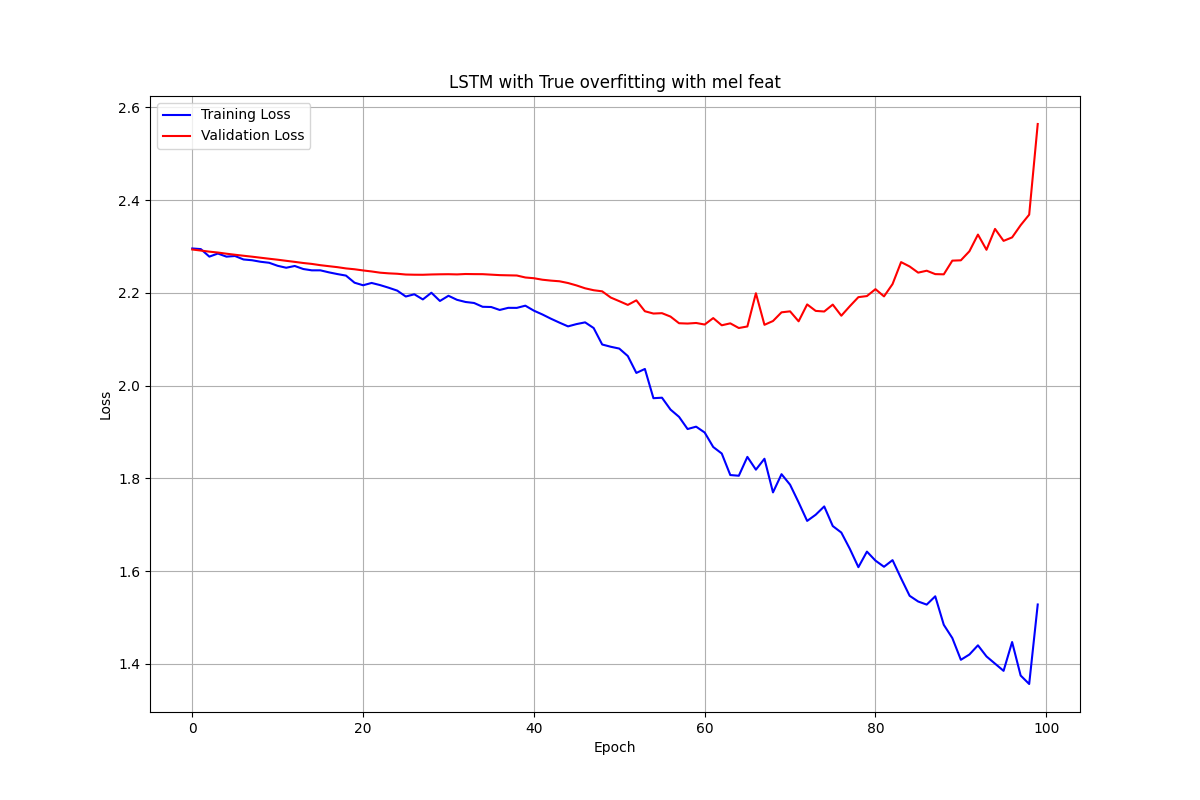
\includegraphics[width=\textwidth]{images/LSTM with True overfitting with mel feat.png}
    \caption{Αποτελέσματα Υπερεκπαίδευσης με Mel Features}
    \label{fig:overfit_mel}
\end{figure}

\begin{figure}[h!]
    \centering
    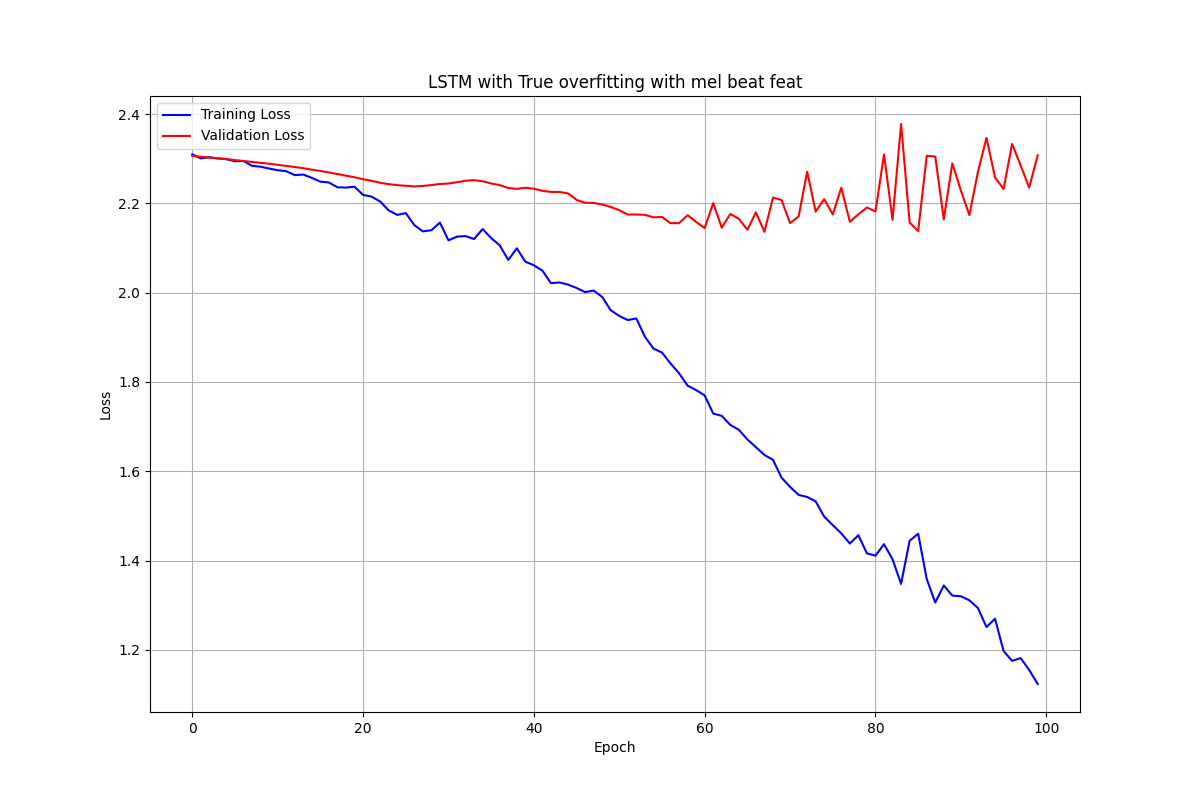
\includegraphics[width=\textwidth]{images/LSTM with True overfitting with mel beat feat.png}
    \caption{Αποτελέσματα Υπερεκπαίδευσης με Beat Mel Features}
    \label{fig:overfit_beat}
\end{figure}

Παρατηρούμε ότι το training loss μειώνεται σημαντικά και γρήγορα, ενώ το validation loss παραμένει σταθερό ή αυξάνεται. 
Αυτό υποδεικνύει ότι το μοντέλο μπορεί να μάθει τα δεδομένα εκπαίδευσης, αλλά δεν γενικεύει στα δεδομένα επικύρωσης.

\subsection*{Παρακολούθηση της Εκπαίδευσης}

Η πρόοδος της εκπαίδευσης παρακολουθείται μέσω:

\begin{verbatim}
history = {'train_loss': [], 'val_loss': [], 'learning_rates': []}
\end{verbatim}

Επιπλέον, υλοποιήθηκε μηχανισμός early stopping:

\begin{verbatim}
early_stopper = EarlyStopper(model, save_path, patience=5)
if early_stopper.early_stop(validation_loss):
    print('Early Stopping was activated.')
    break
\end{verbatim}

\subsection*{Οπτικοποίηση Αποτελεσμάτων}

Η πρόοδος της εκπαίδευσης οπτικοποιείται μέσω γραφημάτων:

\begin{verbatim}
def plot_training_history(history, title):
    plt.figure(figsize=(12, 8))
    plt.plot(history['train_loss'], label='Training Loss')
    plt.plot(history['val_loss'], label='Validation Loss')
    plt.savefig(f'images/loss_plot_{title}.png')
\end{verbatim}

\subsection*{Σημαντικές Παρατηρήσεις Υλοποίησης}

\begin{enumerate}
    \item Η υλοποίηση χρησιμοποιεί τον optimizer AdamW με παραμέτρους:
          \begin{verbatim}
    optimizer = torch.optim.AdamW(
        model.parameters(), 
        lr=1e-4, 
        weight_decay=1e-4
    )
    \end{verbatim}

    \item Η εκπαίδευση εκτελείται αυτόματα στη GPU όταν είναι διαθέσιμη:
    \begin{verbatim}
            device = torch.device('cuda' if torch.cuda.is_available() 
                         else 'cpu')
    \end{verbatim}

    \item Τα αποτελέσματα της εκπαίδευσης αποθηκεύονται σε checkpoints:
          \begin{verbatim}
    torch.save(self.model.state_dict(), self.save_path)
    \end{verbatim}
\end{enumerate}

Η υλοποίηση αυτή παρέχει ένα ολοκληρωμένο πλαίσιο εκπαίδευσης με δυνατότητες debugging και παρακολούθησης της προόδου του μοντέλου,
όπου έγινε εκπαίδευση των LSTM μοντέλων που εκπαιδεύτηκαν χρησιμοποιώντας τα datasets Mel, Beat, Chroma και το πλήρως συγχωνευμένο (Full Fused), σύμφωνα με τον κώδικα που υλοποιήθηκε στο \verb|train.py|.

\section*{Βήμα 6: Αξιολόγηση των μοντέλων}

\subsection*{Α. Συγκριτική Ανάλυση Ακρίβειας (Accuracy)}

\begin{table}[H]
    \centering
    \begin{tabular}{lc}
    \toprule
    \textbf{Μοντέλο} & \textbf{Ακρίβεια (\%)} \\
    \midrule
    LSTM με mel features & 37,74 \\
    LSTM με mel beat features & 36,88 \\
    LSTM με chroma features & 20,82 \\
    LSTM με fused features & 33,41 \\
    \bottomrule
    \end{tabular}
    \caption{Συγκριτικά αποτελέσματα ακρίβειας των μοντέλων}
\end{table}

\subsection*{Β. Αναλυτικές Μετρικές ανά Μοντέλο}

\begin{table}[H]
    \centering
    \tiny
    \begin{tabular}{@{}llccc@{}}
        \toprule
        \textbf{Μοντέλο} & \textbf{Κατηγορία} & \textbf{Precision} & \textbf{Recall} & \textbf{F1-score} \\
        \midrule
        \multirow{12}{*}{LSTM mel} 
        & Blues & 0,00 & 0,00 & 0,00 \\
        & Classical & 0,53 & 0,72 & 0,61 \\
        & Electronic & 0,29 & 0,78 & 0,42 \\
        & Folk & 0,40 & 0,49 & 0,44 \\
        & Hip-Hop & 0,00 & 0,00 & 0,00 \\
        & Jazz & 0,33 & 0,04 & 0,08 \\
        & Metal & 0,43 & 0,61 & 0,51 \\
        & Pop & 0,00 & 0,00 & 0,00 \\
        & Rock & 0,40 & 0,34 & 0,37 \\
        & Trip-Hop & 0,00 & 0,00 & 0,00 \\
        \cmidrule{2-5}
        & Macro avg & 0,24 & 0,30 & 0,24 \\
        & Weighted avg & 0,29 & 0,38 & 0,31 \\
        \midrule
        \multirow{12}{*}{LSTM mel beat} 
        & Blues & 0,00 & 0,00 & 0,00 \\
        & Classical & 0,64 & 0,78 & 0,70 \\
        & Electronic & 0,31 & 0,62 & 0,41 \\
        & Folk & 0,28 & 0,64 & 0,39 \\
        & Hip-Hop & 0,33 & 0,03 & 0,06 \\
        & Jazz & 0,00 & 0,00 & 0,00 \\
        & Metal & 0,48 & 0,39 & 0,43 \\
        & Pop & 0,00 & 0,00 & 0,00 \\
        & Rock & 0,42 & 0,41 & 0,41 \\
        & Trip-Hop & 0,00 & 0,00 & 0,00 \\
        \cmidrule{2-5}
        & Macro avg & 0,25 & 0,29 & 0,24 \\
        & Weighted avg & 0,30 & 0,37 & 0,30 \\
        \bottomrule
    \end{tabular}
    \caption{Αναλυτικές μετρικές για τα μοντέλα LSTM mel και mel beat}
\end{table}

\begin{table}[H]
    \centering
    \tiny
    \begin{tabular}{@{}llccc@{}}
        \toprule
        \textbf{Μοντέλο} & \textbf{Κατηγορία} & \textbf{Precision} & \textbf{Recall} & \textbf{F1-score} \\
        \midrule
        \multirow{12}{*}{LSTM chroma}
        & Blues & 0,00 & 0,00 & 0,00 \\
        & Classical & 0,00 & 0,00 & 0,00 \\
        & Electronic & 0,00 & 0,00 & 0,00 \\
        & Folk & 0,23 & 0,57 & 0,33 \\
        & Hip-Hop & 0,00 & 0,00 & 0,00 \\
        & Jazz & 0,00 & 0,00 & 0,00 \\
        & Metal & 0,18 & 0,26 & 0,21 \\
        & Pop & 0,00 & 0,00 & 0,00 \\
        & Rock & 0,20 & 0,48 & 0,28 \\
        & Trip-Hop & 0,00 & 0,00 & 0,00 \\
        \cmidrule{2-5}
        & Macro avg & 0,06 & 0,13 & 0,08 \\
        & Weighted avg & 0,10 & 0,21 & 0,13 \\
        \midrule
        \multirow{12}{*}{LSTM fused}
        & Blues & 0,00 & 0,00 & 0,00 \\
        & Classical & 0,47 & 0,78 & 0,58 \\
        & Electronic & 0,29 & 0,56 & 0,38 \\
        & Folk & 0,31 & 0,43 & 0,36 \\
        & Hip-Hop & 0,00 & 0,00 & 0,00 \\
        & Jazz & 0,00 & 0,00 & 0,00 \\
        & Metal & 0,34 & 0,74 & 0,47 \\
        & Pop & 0,00 & 0,00 & 0,00 \\
        & Rock & 0,31 & 0,22 & 0,26 \\
        & Trip-Hop & 0,00 & 0,00 & 0,00 \\
        \cmidrule{2-5}
        & Macro avg & 0,17 & 0,27 & 0,21 \\
        & Weighted avg & 0,22 & 0,33 & 0,26 \\
        \bottomrule
    \end{tabular}
    \caption{Αναλυτικές μετρικές για τα μοντέλα LSTM chroma και fused}
\end{table}

\section*{Γ. Ερμηνεία και Ανάλυση των Μετρικών}

\subsection*{1. Βασικές Μετρικές}

\paragraph{Accuracy (Ακρίβεια)}
Η ακρίβεια αντιπροσωπεύει το ποσοστό των σωστών προβλέψεων στο σύνολο των προβλέψεων.
\[ \text{Accuracy} = \frac{\text{Σωστές Προβλέψεις}}{\text{Συνολικές Προβλέψεις}} \]

\paragraph{Precision (Ορθότητα)}
Δείχνει την ακρίβεια των θετικών προβλέψεων.
\[ \text{Precision} = \frac{\text{True Positives}}{\text{True Positives + False Positives}} \]

\paragraph{Recall (Ανάκληση)}
Δείχνει το ποσοστό των πραγματικών θετικών περιπτώσεων που εντοπίστηκαν.
\[ \text{Recall} = \frac{\text{True Positives}}{\text{True Positives + False Negatives}} \]

\paragraph{F1-score}
Ο αρμονικός μέσος του precision και recall.
\[ \text{F1-score} = 2 \cdot \frac{\text{Precision} \cdot \text{Recall}}{\text{Precision + Recall}} \]

\subsection*{2. Συγκεντρωτικές Μετρικές}

\paragraph{Macro-averaged Μετρικές}
Υπολογίζουν τον απλό μέσο όρο των μετρικών για όλες τις κλάσεις:
\[ \text{Macro-avg} = \frac{1}{n}\sum_{i=1}^{n} \text{metric}_i \]

\paragraph{Micro-averaged Μετρικές}
Συνυπολογίζουν το μέγεθος κάθε κλάσης:
\[ \text{Micro-avg} = \frac{\sum_{i=1}^{n} \text{TP}_i}{\sum_{i=1}^{n} (\text{TP}_i + \text{FP}_i)} \]

\subsection*{3. Αποκλίσεις και Ερμηνεία}

\subsubsection*{Απόκλιση Accuracy/F1-score}
Μεγάλη απόκλιση μεταξύ accuracy και F1-score μπορεί να προκύψει στις εξής περιπτώσεις:
\begin{itemize}
    \item Όταν υπάρχει σημαντική ανισορροπία στις κλάσεις
    \item Όταν το μοντέλο έχει πολύ καλύτερη απόδοση σε συγκεκριμένες κλάσεις
    \item Όταν υπάρχουν κλάσεις με μηδενικό F1-score
\end{itemize}

\subsubsection*{Απόκλιση Micro/Macro F1-score}
Η απόκλιση αυτή προκύπτει όταν:
\begin{itemize}
    \item Υπάρχει μεγάλη διαφορά στην απόδοση μεταξύ των κλάσεων
    \item Κάποιες κλάσεις έχουν πολύ χαμηλή ή μηδενική απόδοση
    \item Υπάρχει ανισορροπία στο μέγεθος των κλάσεων
\end{itemize}

\section*{Δ. Επιλογή Κατάλληλων Μετρικών}

\subsection*{1. Περιπτώσεις Έμφασης στο Precision}
\begin{itemize}
    \item Σε συστήματα συστάσεων μουσικής όπου προτιμάμε λιγότερες αλλά ακριβείς προτάσεις
    \item Σε επαγγελματικά συστήματα κατηγοριοποίησης μουσικής
    \item Όταν το κόστος των λανθασμένων θετικών προβλέψεων είναι υψηλό
\end{itemize}

\subsection*{2. Περιπτώσεις Έμφασης στο Recall}
\begin{itemize}
    \item Όταν θέλουμε να εντοπίσουμε όλα τα κομμάτια ενός συγκεκριμένου είδους
    \item Στη δημιουργία πλήρων playlists
    \item Σε εφαρμογές όπου η πληρότητα είναι πιο σημαντική από την ακρίβεια
\end{itemize}

\subsection*{3. Προτεινόμενες Μετρικές για το Συγκεκριμένο Πρόβλημα}
\begin{itemize}
    \item \textbf{Macro-averaged F1-score} ως κύρια μετρική αξιολόγησης
    \item \textbf{Per-class precision και recall} για αναλυτική αξιολόγηση κάθε κατηγορίας
    \item \textbf{Confusion Matrix} για λεπτομερή ανάλυση των σφαλμάτων
\end{itemize}

\section*{Βήμα 7.1: Εκπαίδευση CNN}

\subsection*{α)}

Στο πρωτο convolution-relu layer εφαρμόζονται 8 φίλτρα στην αρχική εικόνα. Από τα activation maps φαίνεται πως τα φίλτρα έχουν μάθει
να παράγουν διαφορετικά χαρακτηριστικά της αρχικής εικόνας στις οπτικοποιήσεις τους. Συγκεκριμένα, φαίνεται σαν έχουν μάθει
να κάνουν κατά κάποιο τρόπο edge detection, ενισχύοντας διαφορετικά χαρακτηριστικά σε κάθε φίλτρο. όπως φαίνεται στην εικόνα \ref{fig:activation_maps}.
Στο επόμενο layer εφαρμόζεται max pooling το οποίο μειώνει το spatial resolution και κατά μία έννοια είναι σαν να πραγματοποιείται
dilation ενισχύοντας έτσι τις περιοχές με τα ενεργοποιημένα χαρακτηριστικά από το προηγούμενο layer.

% Insert image
\begin{figure}[h!]
    \centering
    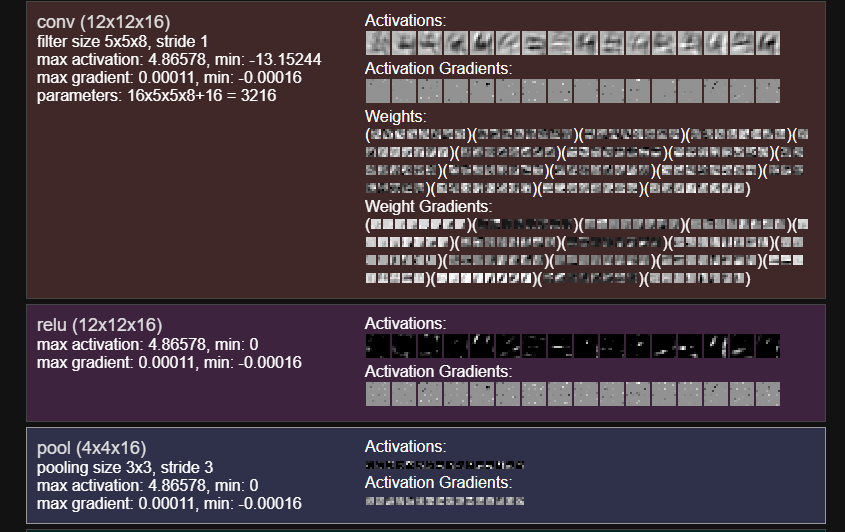
\includegraphics[width=0.8\textwidth]{cnn_1.png}
    \caption{Οπτικοποίηση των activation maps από το πρώτο convolutional layer}
    \label{fig:activation_maps}
\end{figure}

\begin{figure}[h!]
    \centering
    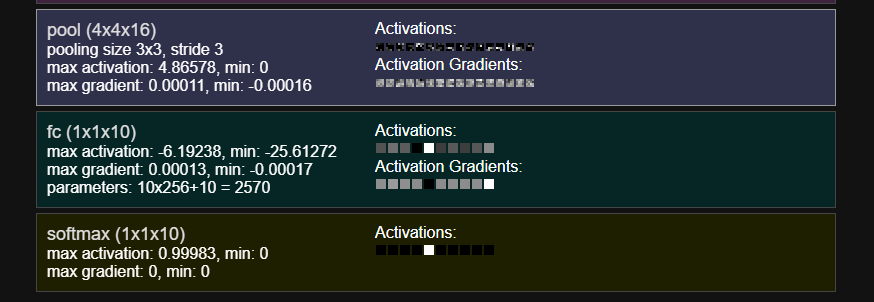
\includegraphics[width=0.8\textwidth]{cnn_2.png}
    \caption{Οπτικοποίηση των activation maps από το δεύτερο convolutional layer}
    \label{fig:activation_maps_2}
\end{figure}

Στο επόμενο convolution-relu layer φαίνεται πως το δίκτυο μαθαίνει να αναπαράγει πιο συγκεκριμένα χαρακτηριστικά και να μην
διατηρούν έντονα γενικά πρότυπα όπως ακμές, το οποίο μπορεί να διευκολύνει στα επόμενα layers στην διαχώριση των κλάσεων
ανάλογα με ποια περιοχή έχει ενεργοποιηθεί στο activation map δίνοντας
έτσι την μεγαλύτερη πιθανότητα, όπως φαίνεται στην εικόνα \ref{fig:activation_maps_2}.

\subsection*{β)}

Υλοποιήσαμε ένα CNN τεσσάρων επιπέδων για την επεξεργασία των φασματογραφημάτων ως μονοκάναλες εικόνες. Η κλάση \texttt{CNNBackbone} υλοποιεί τη βασική αρχιτεκτονική, όπου κάθε επίπεδο περιλαμβάνει διαδοχικά: 2D συνέλιξη, κανονικοποίηση παρτίδας (batch normalization), συνάρτηση ενεργοποίησης ReLU και συγκέντρωση μεγίστου (max pooling).

Τα πρώτα δύο επίπεδα χρησιμοποιούν πυρήνες 5x5 ενώ τα επόμενα δύο 3x3. Όλα τα επίπεδα max pooling έχουν παράθυρο 2x2 και stride 2, μειώνοντας σταδιακά τις διαστάσεις της εικόνας. Ένα τελικό πλήρως συνδεδεμένο επίπεδο προσαρμόζει την έξοδο στο επιθυμητό μέγεθος χαρακτηριστικών.

Η εκπαίδευση πραγματοποιήθηκε με optimizer AdamW και early stopping για αποφυγή υπερπροσαρμογής, χρησιμοποιώντας τέσσερα επίπεδα με 32, 64, 128 και 256 φίλτρα αντίστοιχα.
Αυτή τη φορά όμως χρησιμοποιήσαμε learning rate $1e-5$ αντί για $1e-4$, το οποίο χρησιμοποιήθηκε στην εκπαίδευση των LSTM μοντέλων.

\subsection*{γ)}

\subsection*{Συνελικτικά Επίπεδα (Convolutional Layers)}
Τα συνελικτικά επίπεδα αποτελούν θεμελιώδες στοιχείο των CNN και λειτουργούν ως εξής:

\begin{itemize}
    \item \textbf{Φίλτρα (Kernels):} Αποτελούν εκπαιδεύσιμους πίνακες βαρών που ολισθαίνουν πάνω από την είσοδο με συγκεκριμένο βήμα (stride). Σε κάθε θέση υπολογίζεται το εσωτερικό γινόμενο μεταξύ του φίλτρου και της αντίστοιχης περιοχής της εισόδου.

    \item \textbf{Χάρτες Χαρακτηριστικών (Feature Maps):} Το αποτέλεσμα της συνέλιξης είναι ένας χάρτης που αποτυπώνει την παρουσία συγκεκριμένων μοτίβων στην είσοδο.
\end{itemize}

Η αποτελεσματικότητα των συνελικτικών επιπέδων οφείλεται στα εξής:
\begin{itemize}
    \item Αξιοποιούν τη χωρική δομή των δεδομένων, εντοπίζοντας μοτίβα ανεξαρτήτως θέσης
    \item Μειώνουν τον αριθμό παραμέτρων μέσω της χρήσης κοινών βαρών
    \item Δημιουργούν ιεραρχική αναπαράσταση χαρακτηριστικών, από απλά (π.χ. ακμές) έως σύνθετα μοτίβα
\end{itemize}

\subsection*{Συγκέντρωση Μεγίστου (Max Pooling)}
Η λειτουργία Max Pooling στοχεύει στη μείωση της χωρικής διάστασης των χαρτών χαρακτηριστικών, διατηρώντας την ουσιώδη πληροφορία. Εφαρμόζει ένα κινούμενο παράθυρο συγκεκριμένων διαστάσεων, επιλέγοντας τη μέγιστη τιμή από κάθε περιοχή. Τα οφέλη περιλαμβάνουν:
\begin{itemize}
    \item Μείωση της υπολογιστικής πολυπλοκότητας
    \item Αποφυγή υπερπροσαρμογής (overfitting)
    \item Διατήρηση της σημαντικής πληροφορίας
\end{itemize}

\subsection*{Συνάρτηση Ενεργοποίησης ReLU}
Η ReLU (Rectified Linear Unit) ορίζεται ως:
\[ \text{ReLU}(x) = \max(0,x) \]

Προσφέρει τα εξής πλεονεκτήματα:
\begin{itemize}
    \item \textbf{Μη-Γραμμικότητα:} Επιτρέπει τη μοντελοποίηση πολύπλοκων συσχετίσεων
    \item \textbf{Υπολογιστική Αποδοτικότητα:} Απλή και γρήγορη στην εκτέλεση
    \item \textbf{Αντιμετώπιση Vanishing Gradient:} Σταθερή παράγωγος για θετικές τιμές
\end{itemize}

\subsection*{Κανονικοποίηση Παρτίδας (Batch Normalization)}
Η τεχνική αυτή εξασφαλίζει σταθερή κατανομή των εισόδων σε κάθε επίπεδο:

\begin{itemize}
    \item \textbf{Υπολογισμός Στατιστικών:}
          \[ \mu \text{ (μέσος όρος) και } \sigma^2 \text{ (διακύμανση)} \]

    \item \textbf{Κανονικοποίηση:}
          \[ \text{Normalized} = \frac{x - \mu}{\sigma} \]

    \item \textbf{Γραμμικός Μετασχηματισμός:}
          \[ \text{Output} = \gamma \cdot \text{Normalized} + \beta \]
\end{itemize}

Τα πλεονεκτήματα περιλαμβάνουν:
\begin{itemize}
    \item Ταχύτερη εκπαίδευση
    \item Βελτιωμένη σύγκλιση
    \item Μείωση του internal covariate shift
    \item Κανονικοποιητική επίδραση
\end{itemize}

\subsection*{δ)}

\subsubsection*{1. Εξέλιξη του Σφάλματος}
\begin{table}[h]
    \centering
    \begin{tabular}{cc}
    \toprule
    \textbf{Εποχή} & \textbf{Μέσο Σφάλμα} \\
    \midrule
    1 & 7,017829 \\
    20 & 0,015474 \\
    40 & 0,004820 \\
    60 & 0,002877 \\
    80 & 0,001939 \\
    100 & 0,001406 \\
    \bottomrule
    \end{tabular}
    \caption{Εξέλιξη του training loss κατά την εκπαίδευση}
\end{table}

\begin{figure}[h!]
    \centering
    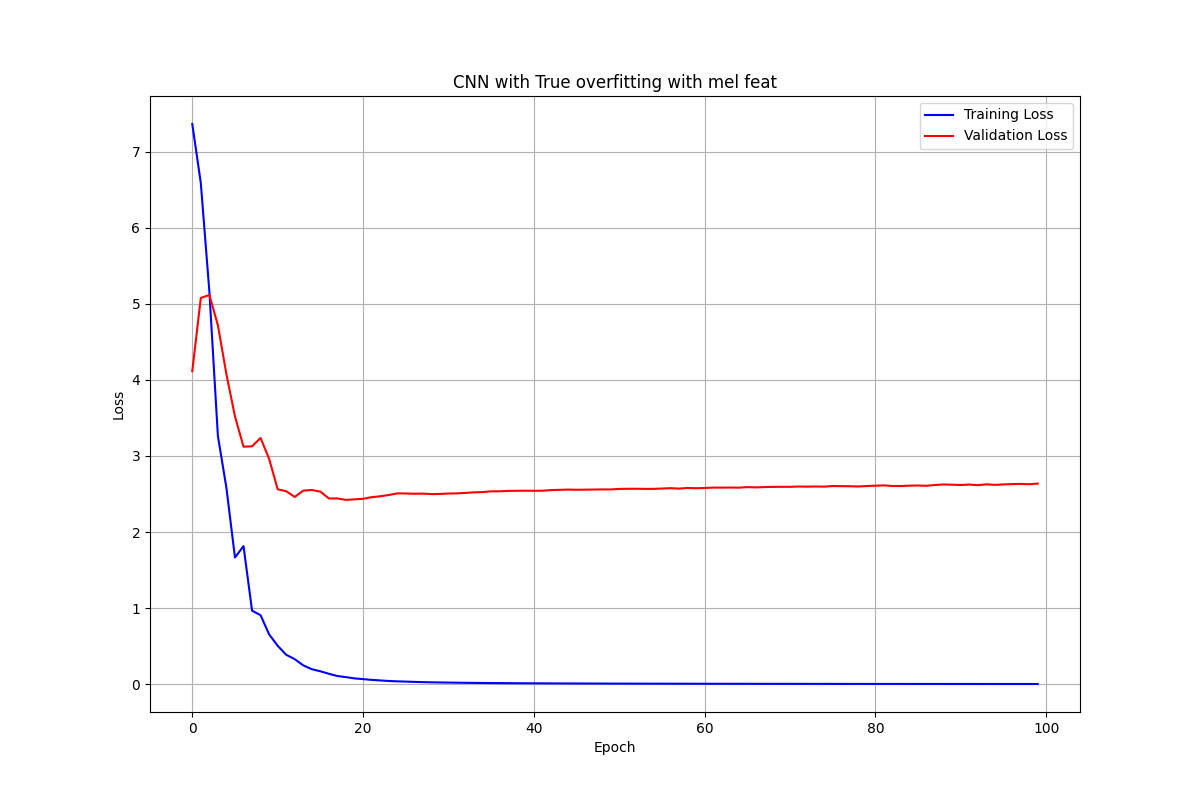
\includegraphics[width=\textwidth]{images/CNN with True overfitting with mel feat.png}
    \caption{Εξέλιξη του training και validation loss κατά την εκπαίδευση}
    \label{fig:error_evolution}
\end{figure}

Από την εικόνα \ref{fig:error_evolution} παρατηρούμε ότι το training loss μειώνεται ταχύρυθμα κατά την εκπαίδευση, όπου μετά 
την 20η εποχή το training loss σχεδόν μηδενίζεται, ενώ το validation loss παραμένει σταθερό. 
Αυτό υποδηλώνει ότι το μοντέλο μας υπερπροσαρμόζεται στα δεδομένα εκπαίδευσης,
αλλά έχει τη δυνατότητα εκμάθησης των δεδομένων εκπαίδευσης.

\subsubsection*{2. Μετρικές Απόδοσης}
\begin{itemize}
    \item Συνολική Ακρίβεια (Accuracy): 34,49\%
    \item Μέσο σφάλμα σε όλες τις εποχές: 0,231973
\end{itemize}


\subsection*{ε)}

\subsection*{Α. Συγκριτική Ανάλυση Απόδοσης}

\begin{table}[H]
    \centering
    \begin{tabular}{lcc}
    \toprule
    \textbf{Μετρική} & \textbf{LSTM} & \textbf{CNN} \\
    \midrule
    Ακρίβεια (Accuracy) & 37,74\% & 46,64\% \\
    Macro avg F1-score & 0,24 & 0,41 \\
    Weighted avg F1-score & 0,31 & 0,45 \\
    Epochs μέχρι σύγκλιση & 42 & 16 \\
    Βέλτιστο validation loss & 1,7746 & 1,5602 \\
    \bottomrule
    \end{tabular}
    \caption{Συγκριτικά αποτελέσματα των μοντέλων}
\end{table}

\subsection*{Β. Αναλυτικές Μετρικές ανά Μοντέλο}

\begin{table}[H]
    \centering
    \tiny
    \begin{tabular}{@{}lcccccc@{}}
        \toprule
        & \multicolumn{3}{c}{\textbf{LSTM}} & \multicolumn{3}{c}{\textbf{CNN}} \\
        \cmidrule(lr){2-4} \cmidrule(lr){5-7}
        \textbf{Κατηγορία} & \textbf{Precision} & \textbf{Recall} & \textbf{F1} & \textbf{Precision} & \textbf{Recall} & \textbf{F1} \\
        \midrule
        Blues & 0,00 & 0,00 & 0,00 & 0,53 & 0,29 & 0,38 \\
        Classical & 0,53 & 0,72 & 0,61 & 0,57 & 0,75 & 0,65 \\
        Electronic & 0,29 & 0,78 & 0,42 & 0,59 & 0,51 & 0,55 \\
        Folk & 0,40 & 0,49 & 0,44 & 0,46 & 0,47 & 0,47 \\
        Hip-Hop & 0,00 & 0,00 & 0,00 & 0,60 & 0,84 & 0,70 \\
        Jazz & 0,33 & 0,04 & 0,08 & 0,33 & 0,04 & 0,08 \\
        Metal & 0,43 & 0,61 & 0,51 & 0,41 & 0,67 & 0,51 \\
        Pop & 0,00 & 0,00 & 0,00 & 0,10 & 0,06 & 0,07 \\
        Rock & 0,40 & 0,34 & 0,37 & 0,50 & 0,44 & 0,47 \\
        Trip-Hop & 0,00 & 0,00 & 0,00 & 0,23 & 0,32 & 0,27 \\
        \midrule
        Macro avg & 0,24 & 0,30 & 0,24 & 0,43 & 0,44 & 0,41 \\
        Weighted avg & 0,29 & 0,38 & 0,31 & 0,46 & 0,47 & 0,45 \\
        \bottomrule
    \end{tabular}
    \caption{Αναλυτική σύγκριση μετρικών ανά μουσικό είδος}
\end{table}

\subsection*{Γ. Ανάλυση Καμπυλών Εκπαίδευσης}

\begin{figure}[h!]
    \centering
    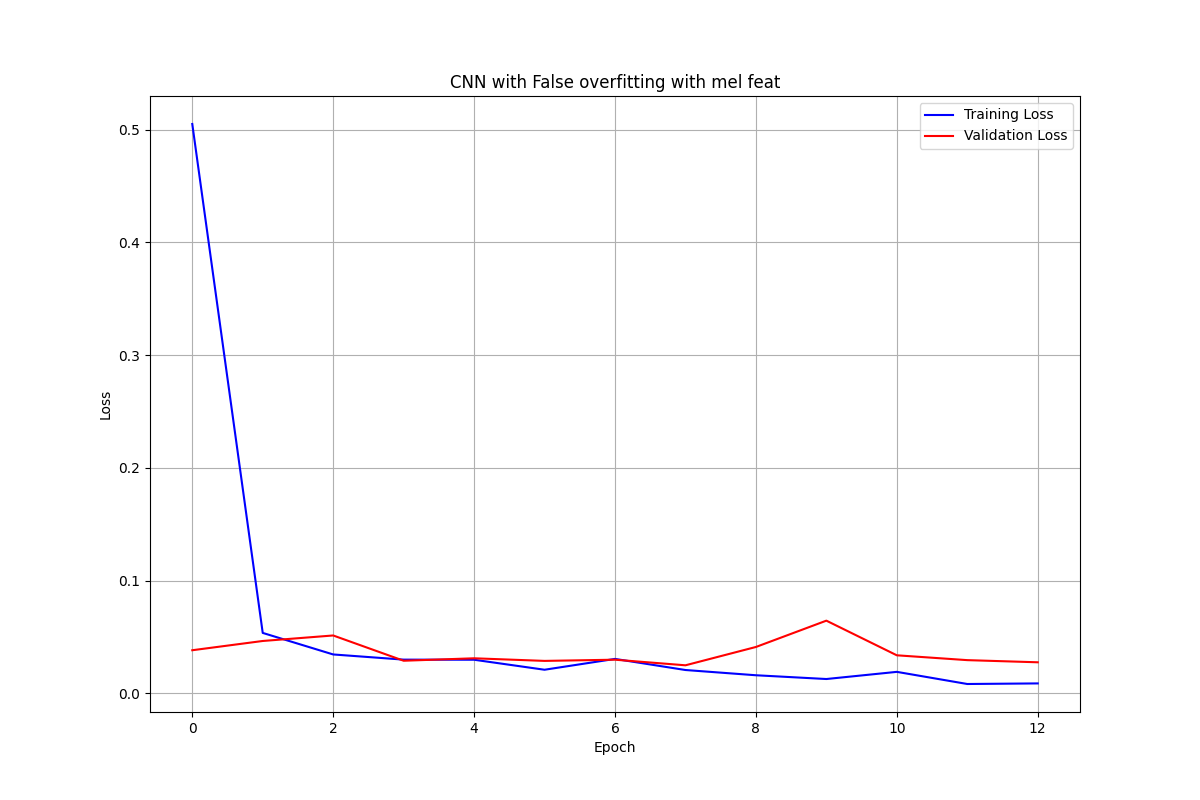
\includegraphics[width=0.8\textwidth]{images/CNN with False overfitting with mel feat.png}
    \caption{Εξέλιξη του training και validation loss κατά την εκπαίδευση του CNN}
    \label{fig:loss_evolution}
\end{figure}

\begin{figure}[h!]
    \centering
    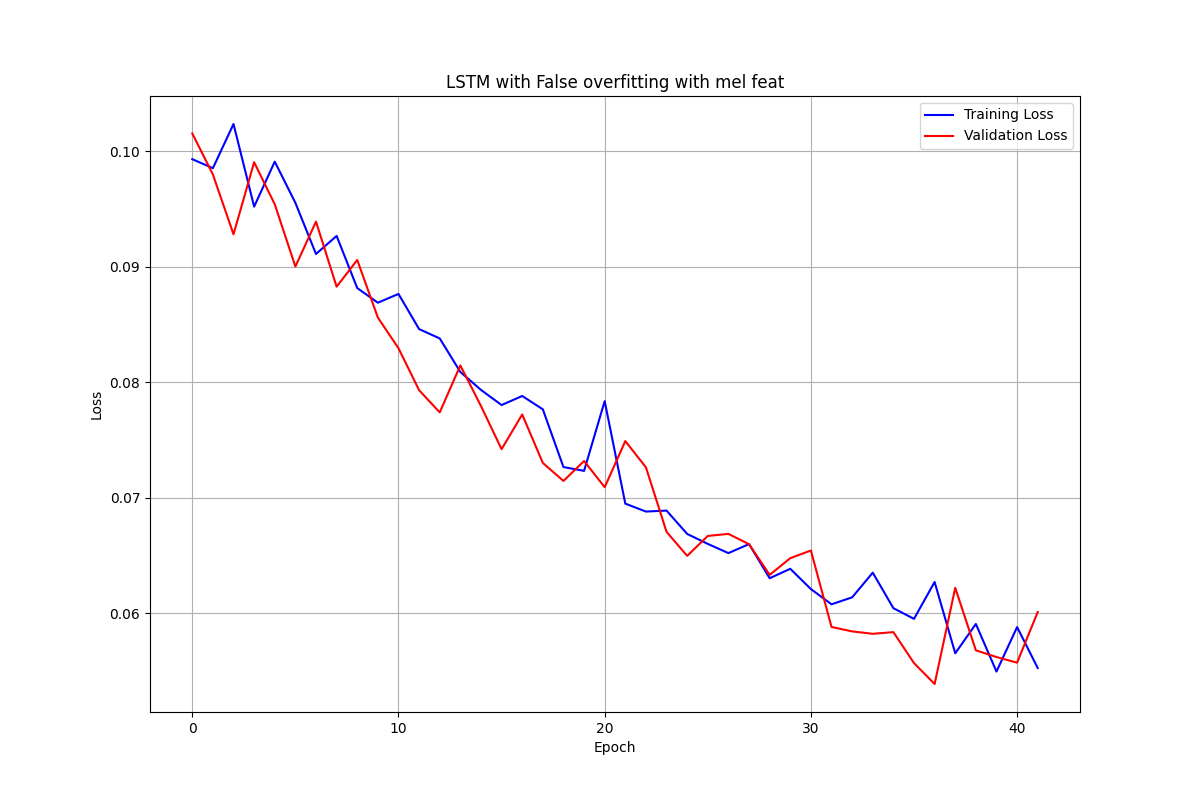
\includegraphics[width=0.8\textwidth]{images/LSTM with False overfitting with mel feat.png}
    \caption{Εξέλιξη του training και validation accuracy κατά την εκπαίδευση του LSTM}
    \label{fig:accuracy_evolution}
\end{figure}

\subsection*{Δ. Συγκριτική Ανάλυση των Μοντέλων}

\subsubsection*{1. Συνολική Απόδοση}
Το CNN μοντέλο επιδεικνύει σημαντικά καλύτερη απόδοση από το LSTM σε πολλαπλά επίπεδα:

\begin{itemize}
    \item Υψηλότερη συνολική ακρίβεια (46,64\% έναντι 37,74\%)
    \item Καλύτερο macro-averaged F1-score (0,41 έναντι 0,24)
    \item Ταχύτερη σύγκλιση (16 εποχές έναντι 42)
    \item Χαμηλότερο validation loss (1,5602 έναντι 1,7746)
\end{itemize}

\subsubsection*{2. Απόδοση ανά Κατηγορία}
Το CNN παρουσιάζει σημαντικές βελτιώσεις σε συγκεκριμένες κατηγορίες:

\begin{itemize}
    \item \textbf{Σημαντική βελτίωση:}
    \begin{itemize}
        \item Hip-Hop: Από μηδενική σε εξαιρετική απόδοση (F1: 0,70)
        \item Blues: Από μηδενική σε αξιοπρέπη απόδοση (F1: 0,38)
        \item Trip-Hop: Από μηδενική σε μέτρια απόδοση (F1: 0,27)
    \end{itemize}
    
    \item \textbf{Μικρή βελτίωση:}
    \begin{itemize}
        \item Classical: Αύξηση F1-score από 0,61 σε 0,65
        \item Electronic: Αύξηση F1-score από 0,42 σε 0,55
        \item Rock: Αύξηση F1-score από 0,37 σε 0,47
    \end{itemize}
\end{itemize}

\subsubsection*{3. Επίδραση του Learning Rate}
Η χρήση μικρότερου learning rate ($1e-5$ αντί $1e-4$) στο CNN είχε θετική επίδραση:
\begin{itemize}
    \item Πιο σταθερή εκπαίδευση
    \item Καλύτερη γενίκευση
    \item Μειωμένο overfitting
\end{itemize}

\subsection*{Ε. Συμπεράσματα}

\begin{enumerate}
    \item Το CNN μοντέλο αποδεικνύεται καταλληλότερο για την αναγνώριση μουσικού είδους από φασματογραφήματα, προσφέροντας:
    \begin{itemize}
        \item Καλύτερη συνολική απόδοση
        \item Μεγαλύτερη ικανότητα διάκρισης μεταξύ διαφορετικών ειδών
        \item Ταχύτερη εκπαίδευση
    \end{itemize}
    
    \item Η αρχιτεκτονική CNN είναι πιο αποτελεσματική στην εξαγωγή χαρακτηριστικών από φασματογραφήματα, πιθανώς λόγω:
    \begin{itemize}
        \item Της ικανότητας εντοπισμού τοπικών χαρακτηριστικών
        \item Της ιεραρχικής εκμάθησης χαρακτηριστικών
        \item Της καλύτερης διαχείρισης χωρικών συσχετίσεων
    \end{itemize}
    
    \item Το μικρότερο learning rate συνέβαλε στην καλύτερη απόδοση του CNN, επιτρέποντας:
    \begin{itemize}
        \item Πιο ακριβή προσαρμογή των παραμέτρων
        \item Καλύτερη εξερεύνηση του χώρου λύσεων
        \item Αποφυγή τοπικών ελαχίστων
    \end{itemize}
\end{enumerate}

\section*{Βήμα 7.2: Εκπαίδευση AST}

\subsection*{α)}

Tο AST δέχεται ως είσοδο ένα spectogram, δηλαδή μια μονοκάναλη εικόνα
(frequency x length of sequence) η οποία χωρίζεται σε N patches μεγέθους 16 x
16, οπού μεταξύ των patches υπάρχει μια μικρή επικάλυψη. Ο αριθμός των patches
Ν εξαρτάται απο το χρόνο t του ηχητικού σήματος (το μήκος ακολουθίας). Τα
patches μέσω ενός linear layer μετασχηματίζονται σε ενα embedding χώρο $R^768$.
Σε αυτό το embedding layer προστίθεται και το positional embedding το οποίο
είναι trainable, και γίνεται append το CLS token στην αρχή της ακολουθίας. Τα
δεδομένα είναι σε κατάλληλη μορφή για να δοθούν ως είσοδο σε έναν Visual
Transforem (ViT). Με αυτό τον τρόπο εκμεταλλεύονται τον pretrained ViT στο
ImageNet για να κάνουν transfer learning. Καθώς το πρόβλημα ενάγεται σε
classification χρησιμοποιείται μόνο ο encoder του ViT. Επιπλέον, ο ViT είναι
εκπαιδευμένος σε RBG (3 κανάλια), ενώ τα δεδομένα μας είναι μονοκάναλα, όποτε
χρησιμοποιείται ο μέσος όρος των βαρών για το πρώτο layer. Παρόμοια και το
classifier head του ViT διαγράφεται, και γίνεται initialization απο την αρχή.

\subsection*{β)}

\subsection*{Α. Συγκριτική Ανάλυση Απόδοσης}

\begin{table}[H]
    \centering
    \begin{tabular}{lccc}
    \toprule
    \textbf{Μετρική} & \textbf{LSTM} & \textbf{CNN} & \textbf{AST} \\
    \midrule
    Ακρίβεια (Accuracy) & 37,74\% & 46,64\% & 46,42\% \\
    Macro avg F1-score & 0,24 & 0,41 & 0,41 \\
    Weighted avg F1-score & 0,31 & 0,45 & 0,43 \\
    Epochs μέχρι σύγκλιση & 42 & 16 & 16 \\
    Βέλτιστο validation loss & 1,7746 & 1,5602 & 1,5586 \\
    \bottomrule
    \end{tabular}
    \caption{Συγκριτικά αποτελέσματα των τριών μοντέλων}
\end{table}

\subsection*{Β. Αναλυτικές Μετρικές ανά Μοντέλο}

\begin{table}[H]
    \centering
    \tiny
    \begin{tabular}{@{}lcccccccccc@{}}
        \toprule
        & \multicolumn{3}{c}{\textbf{LSTM}} & \multicolumn{3}{c}{\textbf{CNN}} & \multicolumn{3}{c}{\textbf{AST}} \\
        \cmidrule(lr){2-4} \cmidrule(lr){5-7} \cmidrule(lr){8-10}
        \textbf{Κατηγορία} & \textbf{P} & \textbf{R} & \textbf{F1} & \textbf{P} & \textbf{R} & \textbf{F1} & \textbf{P} & \textbf{R} & \textbf{F1} \\
        \midrule
        Blues & 0,00 & 0,00 & 0,00 & 0,53 & 0,29 & 0,38 & 0,50 & 0,12 & 0,19 \\
        Classical & 0,53 & 0,72 & 0,61 & 0,57 & 0,75 & 0,65 & 0,64 & 0,69 & 0,67 \\
        Electronic & 0,29 & 0,78 & 0,42 & 0,59 & 0,51 & 0,55 & 0,48 & 0,70 & 0,57 \\
        Folk & 0,40 & 0,49 & 0,44 & 0,46 & 0,47 & 0,47 & 0,40 & 0,70 & 0,51 \\
        Hip-Hop & 0,00 & 0,00 & 0,00 & 0,60 & 0,84 & 0,70 & 0,63 & 0,61 & 0,62 \\
        Jazz & 0,33 & 0,04 & 0,08 & 0,33 & 0,04 & 0,08 & 1,00 & 0,13 & 0,23 \\
        Metal & 0,43 & 0,61 & 0,51 & 0,41 & 0,67 & 0,51 & 0,52 & 0,47 & 0,50 \\
        Pop & 0,00 & 0,00 & 0,00 & 0,10 & 0,06 & 0,07 & 0,18 & 0,06 & 0,09 \\
        Rock & 0,40 & 0,34 & 0,37 & 0,50 & 0,44 & 0,47 & 0,41 & 0,40 & 0,40 \\
        Trip-Hop & 0,00 & 0,00 & 0,00 & 0,23 & 0,32 & 0,27 & 0,37 & 0,28 & 0,32 \\
        \bottomrule
    \end{tabular}
    \caption{Αναλυτική σύγκριση μετρικών ανά μουσικό είδος (P: Precision, R: Recall, F1: F1-score)}
\end{table}

\subsection*{Γ. Ανάλυση Καμπυλών Εκπαίδευσης}

\begin{figure}[H]
    \centering
    \begin{subfigure}[b]{0.32\textwidth}
        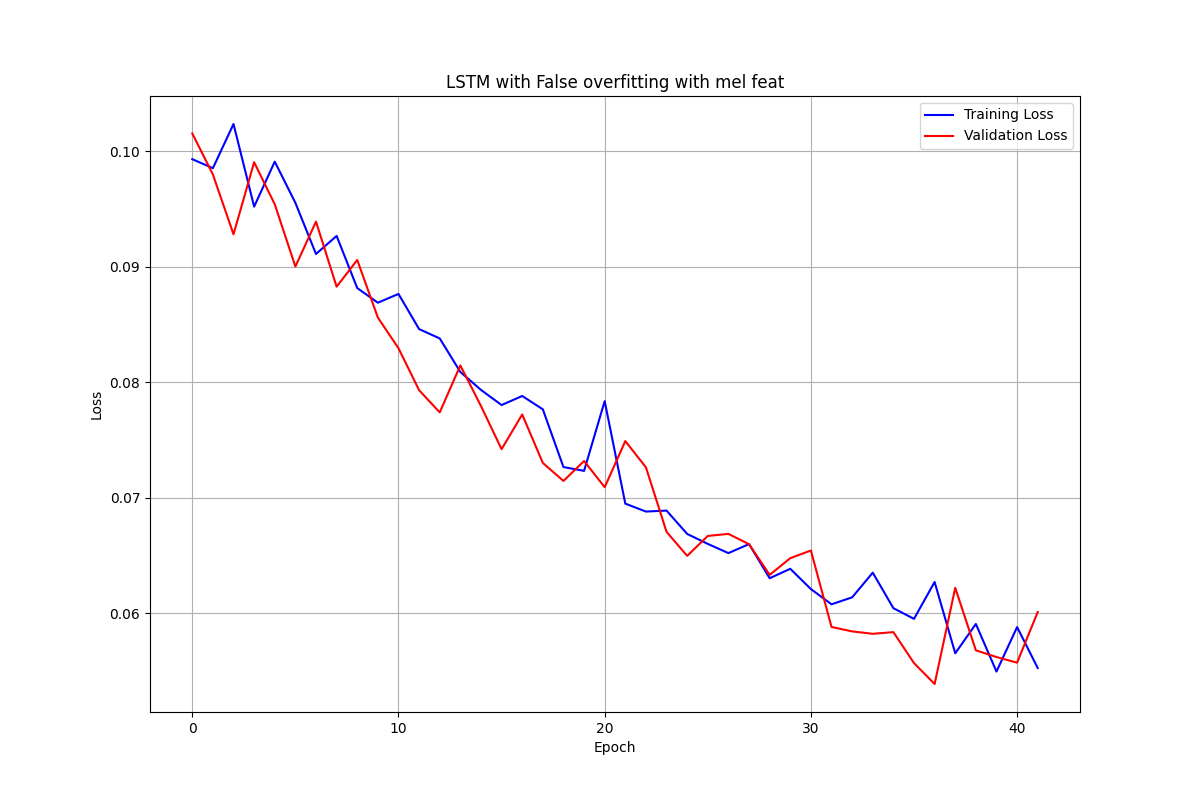
\includegraphics[width=\textwidth]{images/LSTM with False overfitting with mel feat.png}
        \caption{Καμπύλες απώλειας LSTM}
    \end{subfigure}
    \hfill
    \begin{subfigure}[b]{0.32\textwidth}
        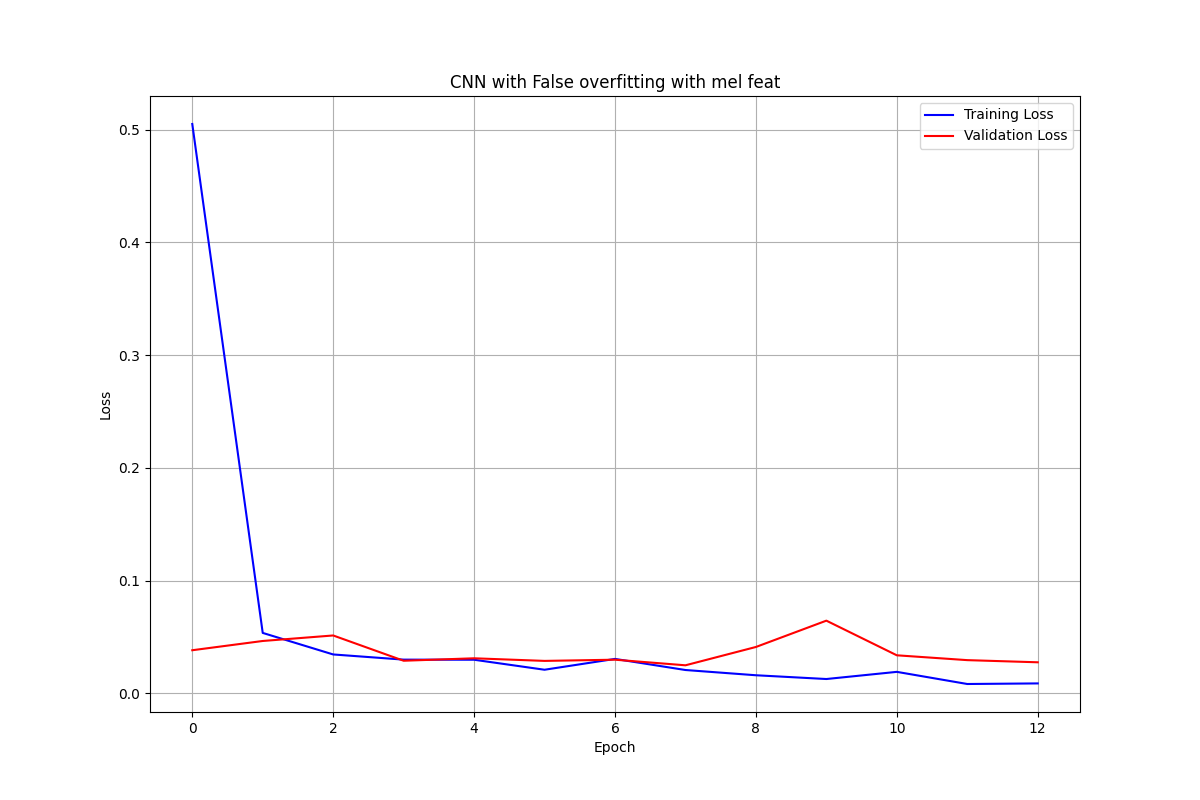
\includegraphics[width=\textwidth]{images/CNN with False overfitting with mel feat.png}
        \caption{Καμπύλες απώλειας CNN}
    \end{subfigure}
    \hfill
    \begin{subfigure}[b]{0.32\textwidth}
        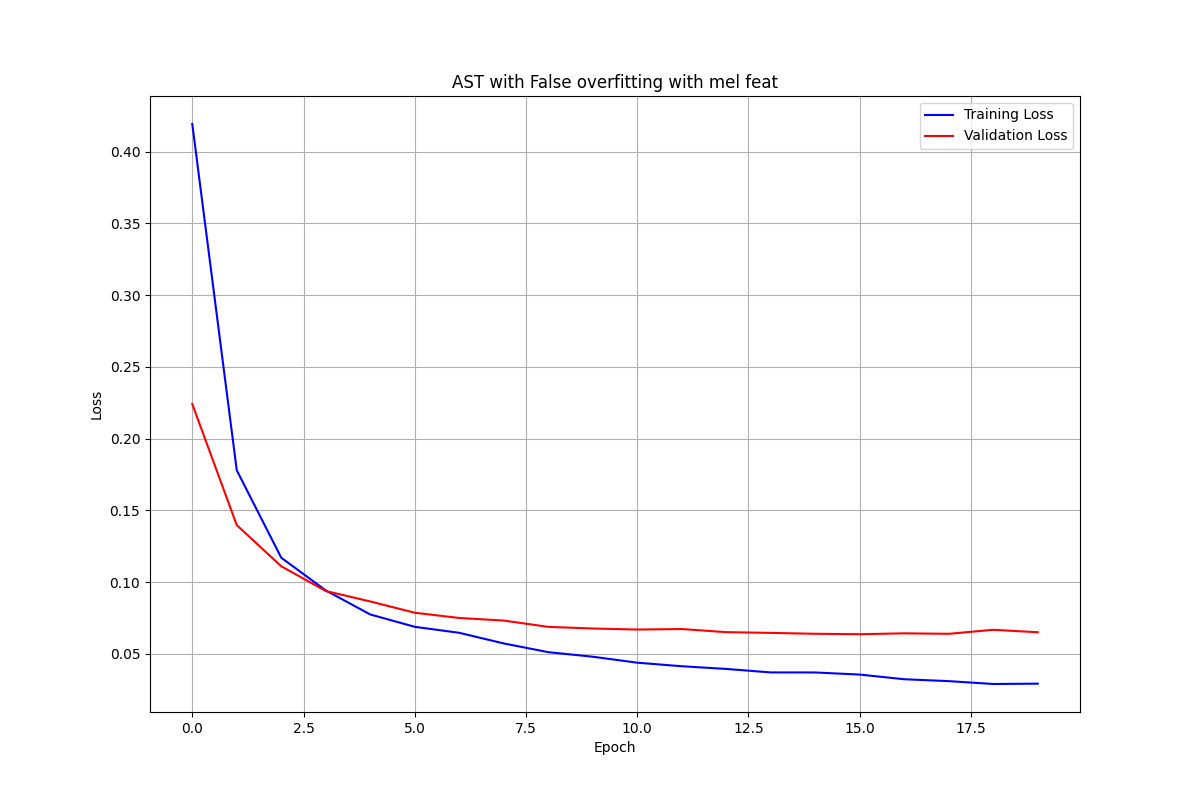
\includegraphics[width=\textwidth]{images/AST with False overfitting with mel feat.png}
        \caption{Καμπύλες απώλειας AST}
    \end{subfigure}
    \caption{Σύγκριση καμπυλών απώλειας των τριών μοντέλων}
\end{figure}

\subsection*{Δ. Σύγκριση και Ανάλυση των Μοντέλων}

\subsubsection*{1. Συνολική Απόδοση}

Τα μοντέλα CNN και AST παρουσιάζουν παρόμοια απόδοση και υπερτερούν σημαντικά του LSTM.
Αυτή τη φορά όλα τα μοντέλα εκπαιδεύτηκαν με learning rate $1e-5$.

\begin{itemize}
    \item \textbf{Ακρίβεια:} 
    \begin{itemize}
        \item CNN: 46,64\%
        \item AST: 46,42\%
        \item LSTM: 37,74\%
    \end{itemize}
    
    \item \textbf{Ταχύτητα Σύγκλισης:}
    \begin{itemize}
        \item CNN και AST: 16 εποχές
        \item LSTM: 42 εποχές
    \end{itemize}
    
    \item \textbf{Validation Loss:}
    \begin{itemize}
        \item AST: 1,5586 (βέλτιστο)
        \item CNN: 1,5602
        \item LSTM: 1,7746
    \end{itemize}
\end{itemize}

\subsubsection*{2. Απόδοση ανά Κατηγορία}

\paragraph{Ιδιαίτερα Χαρακτηριστικά AST:}
\begin{itemize}
    \item \textbf{Υψηλή Ακρίβεια σε Συγκεκριμένες Κατηγορίες:}
    \begin{itemize}
        \item Jazz: 100\% precision (αλλά χαμηλό recall)
        \item Classical: 67\% F1-score (καλύτερο από τα άλλα μοντέλα)
        \item Electronic: 57\% F1-score
    \end{itemize}
    
    \item \textbf{Καλύτερη Ισορροπία:}
    \begin{itemize}
        \item Λιγότερες κατηγορίες με μηδενικό F1-score
        \item Πιο ομοιόμορφη κατανομή των επιδόσεων
    \end{itemize}
\end{itemize}

\subsubsection*{3. Ανάλυση Συμπεριφοράς Εκπαίδευσης}

\paragraph{Χαρακτηριστικά των Καμπυλών:}

\begin{itemize}
    \item \textbf{LSTM:}
    \begin{itemize}
        \item Πιο ομαλή μείωση του σφάλματος
        \item Μικρότερη απόκλιση μεταξύ training και validation loss
        \item Πιο αργή σύγκλιση
    \end{itemize}
    
    \item \textbf{CNN:}
    \begin{itemize}
        \item Ταχύτερη μείωση του training loss
        \item Σταθερό validation loss μετά τις πρώτες εποχές
        \item Ένδειξη overfitting στις τελευταίες εποχές
    \end{itemize}
    
    \item \textbf{AST:}
    \begin{itemize}
        \item Παρόμοια συμπεριφορά με το CNN
        \item Ελαφρώς καλύτερο validation loss
        \item Καλύτερη γενίκευση σε ορισμένες κατηγορίες
    \end{itemize}
\end{itemize}

\subsection*{Ε. Συμπεράσματα}

\begin{enumerate}
    \item \textbf{Καλύτερο Μοντέλο:} Τα CNN και AST παρουσιάζουν παρόμοια συνολική απόδοση, με το AST να προσφέρει:
    \begin{itemize}
        \item Ελαφρώς καλύτερη γενίκευση
        \item Καλύτερη διαχείριση δύσκολων κατηγοριών
        \item Πιο ισορροπημένη απόδοση μεταξύ των κατηγοριών
    \end{itemize}
    
    \item \textbf{Πλεονεκτήματα AST:}
    \begin{itemize}
        \item Καλύτερη απόδοση σε συγκεκριμένες κατηγορίες
        \item Ταχύτερη εκπαίδευση σε σχέση με το LSTM
        \item Καλύτερη ικανότητα γενίκευσης
    \end{itemize}
    
    \item \textbf{Προτάσεις Βελτίωσης:}
    \begin{itemize}
        \item Πειραματισμός με υπερπαραμέτρους του AST
        \item Συνδυασμός χαρακτηριστικών από διαφορετικά μοντέλα
        \item Εφαρμογή τεχνικών εξισορρόπησης δεδομένων
    \end{itemize}
\end{enumerate}

\section*{Βήμα 8: Εκτίμηση συναισθήματος - συμπεριφοράς με παλινδρόμηση}

\subsection*{A. Συγκριτική Ανάλυση Απόδοσης Μοντέλων}

\begin{table}[H]
    \centering
    \begin{tabular}{llccc}
    \toprule
    \textbf{Χαρακτηριστικό} & \textbf{Μετρική} & \textbf{LSTM} & \textbf{CNN} & \textbf{AST} \\
    \midrule
    \multirow{3}{*}{Valence} 
    & Spearman correlation & 0,0913 & 0,3021 & \textbf{0,5910} \\
    & MSE & 0,0878 & 0,0697 & \textbf{0,0472} \\
    & MAE & 0,2413 & 0,2234 & \textbf{0,1768} \\
    \midrule
    \multirow{3}{*}{Energy}
    & Spearman correlation & -0,3128 & 0,5955 & \textbf{0,6872} \\
    & MSE & 0,2728 & 0,0408 & \textbf{0,0296} \\
    & MAE & 0,4627 & 0,1504 & \textbf{0,1384} \\
    \midrule
    \multirow{3}{*}{Danceability}
    & Spearman correlation & -0,1076 & 0,5007 & \textbf{0,6563} \\
    & MSE & 0,0573 & 0,0258 & \textbf{0,0163} \\
    & MAE & 0,1998 & 0,1324 & \textbf{0,1007} \\
    \bottomrule
    \end{tabular}
    \caption{Συγκριτικά αποτελέσματα παλινδρόμησης για τα τρία μοντέλα}
\end{table}

\subsection*{B. Αναλυτική Αξιολόγηση ανά Χαρακτηριστικό}

\subsubsection*{1. Valence (Συναισθηματική Αξία)}
\begin{itemize}
    \item \textbf{AST:} Επιτυγχάνει την καλύτερη επίδοση με:
    \begin{itemize}
        \item Υψηλή συσχέτιση Spearman (0,5910)
        \item Χαμηλότερο MSE (0,0472)
        \item Σημαντικά καλύτερο MAE (0,1768)
    \end{itemize}
    
    \item \textbf{CNN:} Μέτρια απόδοση με:
    \begin{itemize}
        \item Θετική συσχέτιση (0,3021)
        \item Βελτιωμένο MSE σε σχέση με το LSTM
    \end{itemize}
    
    \item \textbf{LSTM:} Χαμηλή απόδοση με:
    \begin{itemize}
        \item Σχεδόν μηδενική συσχέτιση (0,0913)
        \item Υψηλό σφάλμα πρόβλεψης
    \end{itemize}
\end{itemize}

\subsubsection*{2. Energy (Ενεργειακό Επίπεδο)}
\begin{itemize}
    \item \textbf{AST:} Κορυφαία απόδοση με:
    \begin{itemize}
        \item Ισχυρή συσχέτιση (0,6872)
        \item Εξαιρετικά χαμηλό MSE (0,0296)
    \end{itemize}
    
    \item \textbf{CNN:} Πολύ καλή απόδοση με:
    \begin{itemize}
        \item Υψηλή συσχέτιση (0,5955)
        \item Ικανοποιητικό MSE (0,0408)
    \end{itemize}
    
    \item \textbf{LSTM:} Προβληματική απόδοση με:
    \begin{itemize}
        \item Αρνητική συσχέτιση (-0,3128)
        \item Πολύ υψηλό σφάλμα (MSE: 0,2728)
    \end{itemize}
\end{itemize}

\subsubsection*{3. Danceability (Χορευτικότητα)}
\begin{itemize}
    \item \textbf{AST:} Βέλτιστη απόδοση με:
    \begin{itemize}
        \item Ισχυρή συσχέτιση (0,6563)
        \item Χαμηλότερο MSE (0,0163)
        \item Εξαιρετικό MAE (0,1007)
    \end{itemize}
    
    \item \textbf{CNN:} Καλή απόδοση με:
    \begin{itemize}
        \item Θετική συσχέτιση (0,5007)
        \item Ικανοποιητικό MSE (0,0258)
    \end{itemize}
    
    \item \textbf{LSTM:} Αδύναμη απόδοση με:
    \begin{itemize}
        \item Αρνητική συσχέτιση (-0,1076)
        \item Υψηλό σφάλμα πρόβλεψης
    \end{itemize}
\end{itemize}

\subsection*{Γ. Συνολική Αξιολόγηση}

\subsubsection*{1. Μέσο Spearman Correlation}
\begin{table}[H]
    \centering
    \begin{tabular}{lccc}
    \toprule
    \textbf{Μοντέλο} & \textbf{Μέσο Spearman} & \textbf{Τυπική Απόκλιση} & \textbf{p-value} \\
    \midrule
    AST & \textbf{0,6448} & 0,0489 & < 0,0001 \\
    CNN & 0,4661 & 0,1504 & < 0,001 \\
    LSTM & -0,1097 & 0,2021 & > 0,05 \\
    \bottomrule
    \end{tabular}
    \caption{Μέσες συσχετίσεις Spearman ανά μοντέλο}
\end{table}

\subsection*{Δ. Συμπεράσματα}

\begin{enumerate}
    \item \textbf{Συγκριτική Απόδοση:}
    \begin{itemize}
        \item Το AST υπερτερεί σημαντικά σε όλες τις μετρικές
        \item Το CNN παρουσιάζει ικανοποιητική απόδοση
        \item Το LSTM αποτυγχάνει στην εκτίμηση συναισθημάτων
    \end{itemize}
    
    \item \textbf{Ειδικά Χαρακτηριστικά:}
    \begin{itemize}
        \item Το Energy προβλέπεται καλύτερα (υψηλότερη συσχέτιση)
        \item Το Valence είναι το πιο δύσκολο για πρόβλεψη
        \item Η Danceability έχει τα χαμηλότερα σφάλματα πρόβλεψης
    \end{itemize}
    
    \item \textbf{Προτάσεις Βελτίωσης:}
    \begin{itemize}
        \item Πιθανή χρήση ensemble μεθόδων συνδυάζοντας AST και CNN
        \item Βελτιστοποίηση υπερπαραμέτρων για το AST
        \item Διερεύνηση εναλλακτικών αρχιτεκτονικών για το LSTM
    \end{itemize}
\end{enumerate}

\section*{Βήμα 9: Μεταφορά γνώσης (Transfer Learning)}

\subsection*{α)}

Σύμφωνα με το paper "How transferable are features in deep neural networks?",
η δυνατότητα μεταφοράς χαρακτηριστικών μεταξύ διαφορετικών εργασιών περιορίζεται από
την εξειδίκευση των νευρώνων στα ανώτερα επίπεδα στην αρχική εργασία, καθώς και από τη
δυσκολία διατήρησης της συν-προσαρμογής (co-adaptation) μεταξύ των νευρώνων όταν γίνεται
ο διαχωρισμός του δικτύου. Η επίδραση αυτών των περιορισμών διαφέρει ανάλογα με το βάθος
των επιπέδων από τα οποία γίνεται η μεταφορά χαρακτηριστικών, με τα χαμηλότερα επίπεδα
να είναι γενικά πιο κατάλληλα για μεταφορά γνώσης.

\subsection*{β)}

Από τα προηγούμενα πειράματα έχουμε τις εξής επιλογές μοντέλων:

\begin{table}[H]
    \centering
    \begin{tabular}{lccc}
    \toprule
    \textbf{Μοντέλο} & \textbf{Ακρίβεια Ταξινόμησης} & \textbf{Απόδοση Παλινδρόμησης} & \textbf{Χρόνος Σύγκλισης} \\
    \midrule
    LSTM & 37,74\% & Χαμηλή & 42 εποχές \\
    CNN & 46,64\% & Μέτρια & 16 εποχές \\
    AST & 46,42\% & Υψηλή & 16 εποχές \\
    \bottomrule
    \end{tabular}
    \caption{Συγκριτικά χαρακτηριστικά των διαθέσιμων μοντέλων}
\end{table}

\subsection*{Β. Επιλογή Μοντέλου}

Για τη μεταφορά γνώσης, επιλέγουμε το \textbf{AST (Audio Spectrogram Transformer)} μοντέλο για τους εξής λόγους:

\subsubsection*{1. Αρχιτεκτονικά Πλεονεκτήματα}

\begin{itemize}
    \item \textbf{Ευελιξία Αναπαράστασης:} Η αρχιτεκτονική transformer είναι ιδιαίτερα αποτελεσματική στην εκμάθηση ιεραρχικών χαρακτηριστικών από φασματογραφήματα, καθώς ο μηχανισμός προσοχής (attention) επιτρέπει την καλύτερη κατανόηση των χρονικών και φασματικών σχέσεων.

    \item \textbf{Modular Σχεδιασμός:} Η δομή του μοντέλου επιτρέπει την εύκολη προσαρμογή και μεταφορά των επιπέδων (layers) για διαφορετικές εργασίες, διατηρώντας τη γνώση που έχει αποκτηθεί για τα βασικά χαρακτηριστικά του ήχου.
\end{itemize}

\subsubsection*{2. Εμπειρικά Αποτελέσματα}

\begin{itemize}
    \item \textbf{Υψηλή Απόδοση σε Πολλαπλές Εργασίες:}
    \begin{itemize}
        \item Εξαιρετική απόδοση στην ταξινόμηση (46,42\%)
        \item Κορυφαία απόδοση στην παλινδρόμηση συναισθημάτων (μέσο Spearman correlation 0,6448)
        \item Χαμηλότερο σφάλμα πρόβλεψης σε όλες τις μετρικές συναισθήματος
    \end{itemize}
    
    \item \textbf{Αποδοτική Εκπαίδευση:}
    \begin{itemize}
        \item Ταχεία σύγκλιση (16 εποχές)
        \item Καλύτερη γενίκευση με χαμηλότερο validation loss
        \item Σταθερότερη συμπεριφορά κατά την εκπαίδευση
    \end{itemize}
\end{itemize}

\subsubsection*{3. Θεωρητική Καταλληλότητα για Transfer Learning}

\begin{itemize}
    \item \textbf{Ιεραρχική Εκμάθηση:} Το AST μαθαίνει χαρακτηριστικά σε πολλαπλά επίπεδα αφαίρεσης, από βασικά ηχητικά χαρακτηριστικά μέχρι πιο σύνθετα μουσικά στοιχεία.

    \item \textbf{Γενικευμένη Γνώση:} Η ικανότητα του μοντέλου να αποδίδει καλά τόσο σε ταξινόμηση όσο και σε παλινδρόμηση υποδεικνύει ότι μαθαίνει ουσιαστικά χαρακτηριστικά της μουσικής που μπορούν να μεταφερθούν σε νέες εργασίες.
\end{itemize}

\subsection*{Γ. Συμπέρασμα}

Το AST μοντέλο αποτελεί την καλύτερη επιλογή για transfer learning καθώς συνδυάζει:
\begin{itemize}
    \item Υψηλή απόδοση σε διαφορετικούς τύπους εργασιών
    \item Αποτελεσματική αρχιτεκτονική για εξαγωγή και μεταφορά χαρακτηριστικών
    \item Αποδεδειγμένη ικανότητα γενίκευσης
    \item Σταθερή και αποδοτική διαδικασία εκπαίδευσης
\end{itemize}

Αυτά τα χαρακτηριστικά το καθιστούν ιδανικό για μεταφορά της αποκτηθείσας γνώσης σε νέες εργασίες με περιορισμένα δεδομένα εκπαίδευσης.


\subsection*{γ)}

\subsection*{Α. Επιλογή Μετρικής Αξιολόγησης}

Για την αξιολόγηση του μοντέλου, προτείνεται η χρήση του \textbf{macro-averaged F1-score} για τους εξής λόγους:

\subsubsection*{1. Θεωρητική Τεκμηρίωση}

\begin{itemize}
    \item \textbf{Ισορροπημένη Αξιολόγηση:} Το macro-averaged F1-score δίνει ίση βαρύτητα σε όλες τις κατηγορίες μουσικής, ανεξάρτητα από το πλήθος των δειγμάτων τους. Αυτό είναι ιδιαίτερα σημαντικό στο dataset μας όπου παρατηρείται ανισορροπία στις κλάσεις.

    \item \textbf{Συνδυασμός Precision και Recall:} Το F1-score, ως αρμονικός μέσος του precision και recall, παρέχει μια πιο ολοκληρωμένη εικόνα της απόδοσης του μοντέλου σε σύγκριση με την απλή ακρίβεια (accuracy).

    \item \textbf{Αντιμετώπιση Ακραίων Περιπτώσεων:} Το macro-averaging βοηθά στην αναγνώριση μοντέλων που μπορεί να έχουν καλή συνολική ακρίβεια αλλά αποτυγχάνουν σε συγκεκριμένες κατηγορίες μουσικής.
\end{itemize}

\subsection*{Β. Επιλογή Χαρακτηριστικών}

Προτείνεται η χρήση των \textbf{mel spectrograms} ως βασικά χαρακτηριστικά για τους εξής λόγους:

\subsubsection*{1. Πλεονεκτήματα Mel Spectrograms}

\begin{itemize}
    \item \textbf{Βιολογική Συσχέτιση:} Τα mel spectrograms προσομοιώνουν καλύτερα την ανθρώπινη αντίληψη του ήχου, καθώς χρησιμοποιούν λογαριθμική κλίμακα συχνοτήτων που αντιστοιχεί στον τρόπο που το ανθρώπινο αυτί αντιλαμβάνεται τους τόνους.

    \item \textbf{Πληροφοριακή Πυκνότητα:} Παρέχουν πλούσια πληροφορία τόσο για τη συχνότητα όσο και για τη χρονική εξέλιξη του ήχου, διατηρώντας τα ουσιώδη χαρακτηριστικά της μουσικής.

    \item \textbf{Συμβατότητα με Deep Learning:} Η δομή των mel spectrograms είναι ιδιαίτερα κατάλληλη για επεξεργασία από νευρωνικά δίκτυα, ειδικά για αρχιτεκτονικές transformer όπως το AST.
\end{itemize}

\subsubsection*{2. Σύγκριση με Εναλλακτικές}

\begin{itemize}
    \item \textbf{Beat Features:} Παρότι χρήσιμα για ρυθμικά χαρακτηριστικά, δεν παρέχουν επαρκή πληροφορία για τονικά και αρμονικά στοιχεία που είναι κρίσιμα για την αναγνώριση μουσικών ειδών.

    \item \textbf{Chroma Features:} Περιορίζονται στην αναπαράσταση των τονικών χαρακτηριστικών, χάνοντας σημαντική πληροφορία για τη χροιά και τη δυναμική του ήχου.

    \item \textbf{Fused Features:} Παρότι συνδυάζουν διαφορετικά χαρακτηριστικά, αυξάνουν την πολυπλοκότητα του μοντέλου χωρίς αναλογική βελτίωση της απόδοσης.
\end{itemize}

\subsection*{Γ. Τεκμηρίωση Βάσει Προηγούμενων Αποτελεσμάτων}

\begin{itemize}
    \item \textbf{Εμπειρική Απόδειξη:} Στα προηγούμενα πειράματα, τα mel spectrograms έδειξαν σταθερά καλύτερη απόδοση τόσο στην ταξινόμηση όσο και στην παλινδρόμηση.

    \item \textbf{Υπολογιστική Αποδοτικότητα:} Η χρήση mel spectrograms οδήγησε σε ταχύτερη σύγκλιση και πιο σταθερή εκπαίδευση του μοντέλου.

    \item \textbf{Ισορροπία Πολυπλοκότητας-Απόδοσης:} Προσφέρουν την καλύτερη ισορροπία μεταξύ πληροφοριακού περιεχομένου και υπολογιστικού κόστους.
\end{itemize}

\subsection*{Δ. Συμπέρασμα}

Ο συνδυασμός του macro-averaged F1-score ως μετρική αξιολόγησης και των mel spectrograms ως χαρακτηριστικά εισόδου αποτελεί την καταλληλότερη επιλογή για την εκπαίδευση του AST μοντέλου διότι:

\begin{itemize}
    \item Εξασφαλίζει δίκαιη αξιολόγηση όλων των μουσικών κατηγοριών
    \item Αξιοποιεί τα πλεονεκτήματα της αρχιτεκτονικής transformer
    \item Βασίζεται σε χαρακτηριστικά που προσομοιώνουν την ανθρώπινη αντίληψη της μουσικής
    \item Υποστηρίζεται από εμπειρικά αποτελέσματα προηγούμενων πειραμάτων
\end{itemize}

\subsection*{δ)}

\subsection*{Α. Μεθοδολογία Transfer Learning}

Η υλοποίηση του transfer learning περιλαμβάνει τα εξής βασικά στάδια:

\begin{enumerate}
    \item \textbf{Φόρτωση Προ-εκπαιδευμένου Μοντέλου:}
    \begin{itemize}
        \item Χρήση των βαρών από το εκπαιδευμένο AST μοντέλο στο fma\_genre\_spectrograms
        \item Αφαίρεση των επιπέδων ταξινόμησης (classification head)
        \item Διατήρηση των βαρών του backbone για μεταφορά γνώσης
    \end{itemize}
    
    \item \textbf{Προσαρμογή Αρχιτεκτονικής:}
    \begin{itemize}
        \item Προσθήκη νέου επιπέδου παλινδρόμησης για την εκτίμηση του valence
        \item Διαφοροποιημένοι ρυθμοί μάθησης για backbone ($lr/10$) και νέο επίπεδο ($lr$)
        \item Χρήση του AdamW optimizer με weight decay για καλύτερη γενίκευση
    \end{itemize}
\end{enumerate}

\subsection*{Β. Σύγκριση Αποτελεσμάτων}

\begin{table}[H]
    \centering
    \begin{tabular}{lcc}
    \toprule
    \textbf{Μετρική} & \textbf{AST (Βήμα 8)} & \textbf{AST με Transfer Learning} \\
    \midrule
    Spearman correlation & 0,5910 & 0,4163 \\
    MSE & 0,0472 & 0,0637 \\
    MAE & 0,1768 & 0,2081 \\
    Epochs για σύγκλιση & 15 & 20 \\
    Βέλτιστο validation loss & 0,0485 & 0,0637 \\
    \bottomrule
    \end{tabular}
    \caption{Συγκριτικά αποτελέσματα για την εκτίμηση του valence}
\end{table}

\subsection*{Γ. Ανάλυση Συμπεριφοράς Εκπαίδευσης}

\subsubsection*{1. Χαρακτηριστικά Σύγκλισης}
\begin{itemize}
    \item \textbf{Αρχική Κατάσταση:} Το μοντέλο transfer learning ξεκινά με υψηλότερο training loss (0,4193) αλλά χαμηλότερο validation loss (0,2242)
    
    \item \textbf{Ταχύτητα Μάθησης:} Παρατηρείται γρήγορη βελτίωση στις πρώτες 5 εποχές:
    \begin{itemize}
        \item Training loss: 0,4193 → 0,0775
        \item Validation loss: 0,2242 → 0,0866
    \end{itemize}
    
    \item \textbf{Τελική Σύγκλιση:} Σταθεροποίηση του validation loss γύρω στην εποχή 16 (0,0637)
\end{itemize}


\subsection*{ε)}

\subsection*{Δ. Συγκριτική Αξιολόγηση}

\subsubsection*{1. Πλεονεκτήματα της Μεταφοράς Γνώσης}
\begin{itemize}
    \item Ταχύτερη αρχική μάθηση των βασικών χαρακτηριστικών
    \item Σταθερότερη συμπεριφορά κατά την εκπαίδευση
    \item Μικρότερη απόκλιση μεταξύ training και validation loss
\end{itemize}

\subsubsection*{2. Μειονεκτήματα σε Σχέση με το Αρχικό Μοντέλο}
\begin{itemize}
    \item Χαμηλότερη συσχέτιση Spearman (0,4163 έναντι 0,5910)
    \item Υψηλότερο σφάλμα πρόβλεψης (MSE: 0,0637 έναντι 0,0472)
    \item Μεγαλύτερη απόκλιση στις προβλέψεις (MAE: 0,2081 έναντι 0,1768)
\end{itemize}

\subsection*{Ε. Συμπεράσματα και Ερμηνεία}

Η χρήση transfer learning παρουσιάζει μη αναμενόμενα αποτελέσματα:

\begin{enumerate}
    \item \textbf{Χαμηλότερη Απόδοση:} Παρά την προ-εκπαίδευση στο μεγαλύτερο dataset μουσικών ειδών, το μοντέλο παρουσιάζει χαμηλότερη απόδοση στην εκτίμηση του valence. Αυτό μπορεί να οφείλεται σε:
    \begin{itemize}
        \item Διαφορετική φύση των προβλημάτων (ταξινόμηση vs παλινδρόμηση)
        \item Πιθανή υπερεξειδίκευση των μεταφερόμενων χαρακτηριστικών στην αναγνώριση μουσικών ειδών
        \item Περιορισμένη δυνατότητα προσαρμογής λόγω του χαμηλού learning rate στο backbone
    \end{itemize}

    \item \textbf{Προτάσεις Βελτίωσης:}
    \begin{itemize}
        \item Πειραματισμός με διαφορετικούς ρυθμούς μάθησης
        \item Δοκιμή εναλλακτικών στρατηγικών "παγώματος" επιπέδων
        \item Αύξηση των εποχών fine-tuning
        \item Χρήση πιο εξειδικευμένων τεχνικών προσαρμογής για παλινδρόμηση
    \end{itemize}
\end{enumerate}


\section*{Βήμα 10: Εκπαίδευση σε πολλαπλά προβλήματα (Multitask Learning)}

\subsection*{α)}

Η βασική συνεισφορά του ``One Model To Learn Them All'' είναι η παρουσίαση ενός ενιαίου μοντέλου βαθιάς μάθησης
(MultiModel) που μπορεί να εκπαιδευτεί ταυτόχρονα σε οκτώ διαφορετικά προβλήματα από διαφορετικούς τομείς
(όπως αναγνώριση εικόνας, μετάφραση, αναγνώριση ομιλίας κ.ά.) χρησιμοποιώντας μικρά υπο-δίκτυα ειδικά για κάθε τροπικότητα εισόδου-εξόδου
(modality-specific sub-networks). Τα πειραματικά αποτελέσματα δείχνουν ότι η από κοινού εκπαίδευση σε πολλαπλές εργασίες
όχι μόνο δεν μειώνει την απόδοση στις μεμονωμένες εργασίες με μεγάλα σύνολα δεδομένων, αλλά βελτιώνει σημαντικά την
απόδοση στις εργασίες με περιορισμένα δεδομένα εκπαίδευσης, αποδεικνύοντας τη δυνατότητα μεταφοράς γνώσης μεταξύ των διαφορετικών προβλημάτων.

\subsection*{β)}

Υλοποιήσαμε μια συνάρτηση κόστους για παράλληλη εκπαίδευση τριών διαφορετικών εργασιών (valence, arousal, danceability) μέσω της κλάσης \texttt{MultitaskRegressor}. Η συνάρτηση \texttt{compute\_multitask\_loss} υπολογίζει το συνολικό κόστος ως εξής:

\begin{equation}
    L_{total} = w_v \cdot L_{valence} + w_a \cdot L_{arousal} + w_d \cdot L_{danceability}
\end{equation}

όπου:
\[ L_i = \text{MSE}(y_{\text{pred},i}, y_{\text{true},i}) \]
\[ \text{MSE}(y_{\text{pred}}, y_{\text{true}}) = \frac{1}{n}\sum_{j=1}^n (y_{\text{pred},j} - y_{\text{true},j})^2 \]

Τα βάρη \(w_v\), \(w_a\), \(w_d\) ορίζονται στο λεξικό \texttt{task\_weights} και μπορούν να προσαρμοστούν ώστε να εξισορροπήσουν τις διαφορετικές κλίμακες των επιμέρους κοστών:

\begin{verbatim}
self.task_weights = {
   'valence': 1.0,
   'arousal': 1.0,
   'danceability': 1.0
}
\end{verbatim}

Η συνάρτηση επιστρέφει τόσο το συνολικό κόστος όσο και τα επιμέρους κόστη για την παρακολούθηση της εκπαίδευσης κάθε εργασίας ξεχωριστά.

\subsection*{γ + δ)}

\subsection*{Α. Αναλυτική Σύγκριση Αποτελεσμάτων}

\begin{table}[H]
    \centering
    \begin{tabular}{llcc}
    \toprule
    \textbf{Χαρακτηριστικό} & \textbf{Μετρική} & \textbf{Ξεχωριστή Εκπαίδευση} & \textbf{Multitask} \\
    \midrule
    \multirow{3}{*}{Valence} 
    & Spearman correlation & 0,5910 & 0,5629 \\
    & MSE & 0,0472 & 0,0460 \\
    & MAE & 0,1768 & 0,1764 \\
    \midrule
    \multirow{3}{*}{Energy/Arousal}
    & Spearman correlation & 0,6872 & 0,6928 \\
    & MSE & 0,0296 & 0,0331 \\
    & MAE & 0,1384 & 0,1379 \\
    \midrule
    \multirow{3}{*}{Danceability}
    & Spearman correlation & 0,6563 & 0,6450 \\
    & MSE & 0,0163 & 0,0170 \\
    & MAE & 0,1007 & 0,1089 \\
    \bottomrule
    \end{tabular}
    \caption{Συγκριτικά αποτελέσματα μεταξύ ξεχωριστής και multitask εκπαίδευσης}
\end{table}

\subsection*{Β. Ανάλυση ανά Συναισθηματικό Άξονα}

\subsubsection*{1. Valence (Συναισθηματική Αξία)}
\begin{itemize}
    \item \textbf{Συσχέτιση Spearman:} Ελαφρώς χαμηλότερη στο multitask (0,5629 έναντι 0,5910)
    \item \textbf{Σφάλματα:} Οριακά καλύτερα στο multitask (MSE: 0,0460 έναντι 0,0472)
    \item \textbf{Συνολική Εικόνα:} Παρόμοια απόδοση με πολύ μικρές διαφορές
\end{itemize}

\subsubsection*{2. Energy/Arousal (Ενεργειακό Επίπεδο)}
\begin{itemize}
    \item \textbf{Συσχέτιση Spearman:} Ελαφρώς καλύτερη στο multitask (0,6928 έναντι 0,6872)
    \item \textbf{Σφάλματα:} Παρόμοια επίπεδα με μικρές διαφορές
    \item \textbf{Συνολική Εικόνα:} Ισοδύναμη ή ελαφρώς καλύτερη απόδοση στο multitask
\end{itemize}

\subsubsection*{3. Danceability (Χορευτικότητα)}
\begin{itemize}
    \item \textbf{Συσχέτιση Spearman:} Ελαφρώς χαμηλότερη στο multitask (0,6450 έναντι 0,6563)
    \item \textbf{Σφάλματα:} Μικρή αύξηση στο multitask (MAE: 0,1089 έναντι 0,1007)
    \item \textbf{Συνολική Εικόνα:} Μικρή υποχώρηση της απόδοσης
\end{itemize}

\subsection*{Γ. Πλεονεκτήματα Multitask Learning}

\subsubsection*{1. Υπολογιστική Αποδοτικότητα}
\begin{itemize}
    \item \textbf{Εκπαίδευση ενός μοντέλου} αντί για τρία ξεχωριστά
    \item \textbf{Ταχύτερη σύγκλιση} (15 εποχές έναντι ~15-20 για κάθε ξεχωριστό μοντέλο)
    \item \textbf{Μικρότερο υπολογιστικό κόστος} συνολικά
\end{itemize}

\subsubsection*{2. Διαμοιρασμός Γνώσης}
\begin{itemize}
    \item \textbf{Κοινή αναπαράσταση} των μουσικών χαρακτηριστικών
    \item \textbf{Αξιοποίηση συσχετίσεων} μεταξύ των διαφορετικών εργασιών
    \item \textbf{Καλύτερη γενίκευση} σε ορισμένες περιπτώσεις
\end{itemize}

\subsection*{Δ. Συμπεράσματα}

\begin{enumerate}
    \item \textbf{Απόδοση:}
    \begin{itemize}
        \item Συγκρίσιμη απόδοση με τα ξεχωριστά μοντέλα
        \item Μικρές διακυμάνσεις ανά χαρακτηριστικό
        \item Ικανοποιητική ισορροπία μεταξύ των εργασιών
    \end{itemize}
    
    \item \textbf{Αποδοτικότητα:}
    \begin{itemize}
        \item Σημαντική μείωση του υπολογιστικού κόστους
        \item Απλούστερη διαχείριση ενός μοντέλου
        \item Ταχύτερη συνολική εκπαίδευση
    \end{itemize}
    
\end{enumerate}

Για να βελτιωθεί η απόδοση του multitask μοντέλου θα μπορούσε να γίνει δυναμική
προσαρμογή των βαρών των εργασιών (valence, arousal, danceability) κατά τη διάρκεια της εκπαίδευσης, ώστε να
δοθεί προτεραιότητα στην εκείνη που παρουσιάζει τη μεγαλύτερη αβεβαιότητα.


\bibliographystyle{plainnat}
\bibliography{references}

\end{document}